\documentclass[ROIA,Unicode]{cedram}

\AtBeginDocument{\inputencoding{utf8}}
\usepackage[numbers,sort&compress]{natbib}
\usepackage{booktabs}
\usepackage{graphicx}
\usepackage{longtable}
\usepackage{tabularx}
\usepackage{xurl}
\usepackage{microtype}

\datereceived{2026-04-17}
\issueinfo{0}{0}{0}{2026}
\SetFirstPage{1}

\makeatletter
\def\@setdates{%
\vglue4mm
\rightline{\itshape\Small
\ifx\@empty\@datereceived\else\@setdatereceived\fi
\ifx\@empty\@daterevised\else\@setdaterevised\fi}}
\makeatother

\makeatletter
\AtBeginDocument{%
\@ifundefined{theHtable}{}{% 
\renewcommand{\theHtable}{\thesection.\arabic{table}}}%
\@ifundefined{theHfigure}{}{% 
\renewcommand{\theHfigure}{\thesection.\arabic{figure}}}%
}
\makeatother

\title[LLM, SHS et épidémiologie]{LLM, SHS et épidémiologie : intégration de profils socio-comportementaux dans un pipeline français de matrices de contact}
\alttitle{LLMs, social sciences and epidemiology: integrating socio-behavioral profiles into a French contact-matrix pipeline}

\author{\firstname{Martin} \lastname{Collins}}
\address{Université Paris 1 Panthéon-Sorbonne, Diplôme d'Université de science des données, Paris, France}
\email{utmostsenior@proton.me}

\keywords{contact matrices, large language models, social sciences, epidemiological modeling, France, socio-behavioral profiles}
\altkeywords{matrices de contact, grands modèles de langage, sciences humaines et sociales, modélisation épidémiologique, France, profils socio-comportementaux}

\subjclass{62P10, 68T07, 91D10}

\emergencystretch=2em

\begin{document}

\begin{abstract}
Age-structured contact matrices are central to epidemic modeling, yet they compress social heterogeneity and rarely articulate how behavioral change should be reintroduced in a transparent way. The paper addresses a specific question: can a socio-behavioral LLM layer enrich a French contact-matrix pipeline without hiding its assumptions behind black-box claims?

We therefore develop an incremental protocol in four stages. First, we compare a minimal demographic rescaling with a contextual baseline structured by home, school, work and community contacts, then optimize this baseline on COMES-F. Second, we add a lightweight temporal behavioral layer calibrated on French CoviPrev and SocialCov series. Third, we introduce 18 explicit socio-demographic profiles and a first campaign of real LLM generations, using Claude Sonnet 4.6, to recover regime ordering and social heterogeneity. Fourth, we make the LLM block more central by turning it into a structured SHS mediation layer, iteratively refined through experiments exp007, exp008 and exp009, with a final campaign on Claude Haiku 4.5 and a revised mobility-oriented prompt.

The static baseline remains useful, but the main result now lies in the LLM block. The first campaign already recovers plausible differences in responsiveness between white-collar and agricultural profiles. More importantly, the exp007 to exp009 sequence shows that the main bottleneck was not the SHS-LLM hypothesis itself, but the calibration of the latent mobility variable. In the final exp009 configuration, the LLM layer outperforms the heuristic benchmark on both mobility and prevention, with a mobility MAE of 0.0219 versus 0.0935, a mobility correlation of 0.989 versus 0.863, and a prevention MAE of 0.0685 versus 0.1409. The contribution is therefore not a claim that LLMs replace survey data, but a transparent and auditable protocol showing how they can be inserted as socio-behavioral mediators between public policy regimes, named social profiles and diffusion-relevant contact modifiers.
\end{abstract}

\begin{altabstract}
Les matrices de contact par âge sont centrales en modélisation épidémiologique, mais elles écrasent souvent une partie des différences sociales de comportement et explicitent rarement la manière de les réintroduire sans opacifier le modèle. Le présent article s'organise autour d'une question précise : une couche LLM socio-comportementale peut-elle enrichir un pipeline français de matrices de contact tout en gardant ses hypothèses visibles et auditables ?

Pour y répondre, nous développons un protocole incrémental en quatre étapes. D'abord, nous comparons une repondération démographique minimale à un socle contextuel structuré par domicile, école, travail et communauté, puis nous optimisons ce socle sur COMES-F. Ensuite, nous ajoutons une couche comportementale temporelle légère calibrée sur les séries françaises CoviPrev et SocialCov. Puis nous introduisons 18 profils socio-démographiques explicites et une première campagne de générations réelles par LLM, avec Claude Sonnet 4.6, afin de restituer l'ordre des régimes sanitaires et une hétérogénéité sociale plausible. Enfin, nous rendons le bloc LLM plus central en le reformulant comme couche de médiation SHS structurée, raffinée itérativement au fil des expériences exp007, exp008 et exp009, avec une campagne finale sur Claude Haiku 4.5 et un prompt révisé centré sur la mobilité.

Le socle statique reste utile, mais le résultat principal se situe désormais dans le bloc LLM. La première campagne fait déjà apparaître des écarts plausibles de réactivité entre profils cadres et profils agricoles. Surtout, la séquence exp007 à exp009 montre que le principal verrou n'était pas l'hypothèse SHS-LLM en elle-même, mais le calibrage de la variable latente de mobilité. Dans la configuration finale exp009, la couche LLM surpasse la référence heuristique à la fois sur la mobilité et sur la prévention, avec une MAE mobilité de 0,0219 contre 0,0935, une corrélation mobilité de 0,989 contre 0,863, et une MAE prévention de 0,0685 contre 0,1409. La contribution n'est donc pas de prétendre que les LLM remplacent les enquêtes, mais de proposer un protocole transparent et auditable montrant comment les insérer comme médiateurs socio-comportementaux entre régimes de politique publique, profils sociaux nommés et modificateurs de contact utiles à la diffusion épidémique.
\end{altabstract}

\maketitle

\section{Introduction}
Ce travail a été réalisé dans le cadre du mémoire du Diplôme d'Université (DU) en science des données de l'Université Paris 1 Panthéon-Sorbonne. Le coeur de l'étude est l'intégration progressive d'un médiateur socio-comportemental explicite entre des régimes de politique publique, des profils sociaux nommés et des modificateurs de contact utiles à la modélisation épidémique.

Les matrices de contact par âge occupent une place décisive dans les modèles de transmission parce qu'elles quantifient la manière dont les groupes d'âge se rencontrent. Elles sont pourtant peu adaptées, en l'état, à la restitution des inégalités sociales de marge de manoeuvre face à une crise sanitaire. Entre une matrice nationale agrégée et une simulation agentique lourde, il manque souvent un niveau intermédiaire capable d'expliciter des profils sociaux, des contraintes de mobilité, des différences de confiance institutionnelle et des capacités inégales d'adhésion aux mesures. C'est précisément cet espace méthodologique que nous cherchons à documenter.

Le cas français s'y prête bien. COMES-F fournit un ancrage empirique robuste pour la structure des contacts \citep{beraud2015french}, tandis que CoviPrev, SocialCov et Google Mobility documentent des transformations temporelles du comportement au cours de la pandémie \citep{coviprev2021,socialcov2024,googlemobility2022}. Mais ces jeux de données ne donnent pas directement une articulation entre structures de contact, positions sociales et réponses comportementales. Notre hypothèse est qu'une couche LLM bornée, profilée et auditée peut jouer ce rôle de médiation, à condition de rester strictement encadrée, comparée à des baselines explicites, et interprétée comme instrument de scénarisation structurée plutôt que comme mesure directe d'un comportement vrai.

Le manuscrit suit donc un ordre de complexité croissante. Nous établissons d'abord un socle statique transparent, puis une couche temporelle calibrable, avant de faire du bloc LLM l'objet central de l'analyse. Cette trajectoire compte scientifiquement, parce qu'elle permet de distinguer ce qui provient d'un meilleur socle structurel, ce qui vient d'une calibration temporelle encore fragile, et ce qui tient à l'introduction d'une médiation socio-comportementale par LLM. Les itérations récentes du projet jouent ici un rôle substantiel. Une première campagne, fondée sur des appels réels à Claude Sonnet 4.6, a montré qu'il était possible de retrouver une hiérarchie plausible des régimes sanitaires et des contrastes sociaux de réactivité. Une seconde série d'expériences, exp007 à exp009, a ensuite révélé que la difficulté majeure se situait moins dans l'idée SHS-LLM elle-même que dans le cadrage de la variable latente \emph{mobility\_reduction}. La version finale exp009, exécutée avec Claude Haiku 4.5 et un protocole de prompt révisé, corrige précisément ce point.

L'article poursuit quatre objectifs. Premièrement, établir un socle français reproductible pour les matrices de contact synthétiques. Deuxièmement, montrer ce qu'une couche comportementale légère apporte, et n'apporte pas, lorsque l'on passe en dynamique temporelle. Troisièmement, tester si des profils socio-démographiques explicites permettent à un LLM de produire des écarts sociaux et des ordres de régimes sanitaires plausibles. Quatrièmement, documenter honnêtement comment la performance du bloc LLM dépend du choix du protocole de médiation, du prompt et du modèle mobilisé. Notre contribution principale n'est donc plus seulement un pipeline incrémental. Elle consiste à rendre visible, traçable et discutable l'intégration d'une couche SHS/LLM dans une chaîne de modélisation épidémiologique française.

\section{Travaux connexes}
Les enquêtes de contacts restent le point de départ le plus convaincant pour décrire les mélanges intergénérationnels pertinents en santé publique. POLYMOD a joué, à cet égard, un rôle fondateur en montrant la robustesse de certains motifs de contact, notamment l'assortativité par âge et l'importance des contextes quotidiens \citep{mossong2008social}. Pour la France, COMES-F a apporté un ancrage empirique décisif en documentant les contacts déclarés, leurs variations selon le calendrier et la nécessité de corriger certains biais de réciprocité \citep{beraud2015french}. Ces travaux constituent davantage qu'une source de comparaison: ils fixent aussi les propriétés minimales qu'une matrice synthétique crédible devrait retrouver, au moins grossièrement.

Une seconde famille de travaux vise moins à mesurer directement les contacts qu'à les projeter dans des pays ou des régions dépourvus d'enquêtes dédiées. Les matrices de Prem et collègues ont ici fait référence, en combinant enquêtes existantes, structures démographiques, organisation scolaire et participation au travail pour produire des matrices synthétiques à large couverture géographique \citep{prem2017projecting,prem2021projecting}. Cette approche est extrêmement utile, et nous en retenons l'idée centrale selon laquelle une décomposition par contextes facilite la transférabilité. En revanche, notre objectif est plus restreint. Il ne s'agit pas de reconstruire un modèle hiérarchique international, mais d'examiner ce que l'on peut obtenir dans un cadre français plus léger, où les hypothèses restent immédiatement inspectables.

Une troisième ligne de recherche pousse la synthèse beaucoup plus loin en construisant des populations artificielles riches, à partir de microdonnées socio-démographiques et de mécanismes explicites d'affectation aux ménages, aux écoles ou aux lieux de travail \citep{mistry2021inferring}. Ces pipelines offrent un réalisme structurel nettement supérieur et ouvrent la voie à des analyses fines, notamment à l'échelle infranationale. Ils exigent toutefois davantage de données, davantage de choix de modélisation et, souvent, une chaîne de validation plus lourde. Notre travail se situe en amont de cette ambition. Il réemploie l'intuition des composantes domicile-école-travail-autres, simplifie fortement la représentation des structures sociales et laisse hors champ, à ce stade, la synthèse complète de populations, la dynamique temporelle détaillée et la modélisation régionale.

Depuis 2023, une littérature distincte explore l'usage des grands modèles de langage comme simulateurs sociaux, agents génératifs ou agents économiques stylisés \citep{park2023generative,argyle2023out,horton2023homo}. Cette littérature montre qu'un LLM peut restituer des hiérarchies d'action plausibles lorsqu'il est ancré dans des rôles ou des contraintes explicites. Elle rappelle aussi que ces dispositifs demeurent fortement dépendants de la formulation des profils, des variables injectées dans les prompts et des biais propres au modèle \citep{weidinger2022taxonomy,bender2021stochastic}. Notre travail reprend cette intuition exploratoire, mais dans un cadre plus borné: profils synthétiques nommés, sorties JSON contraintes, caches archivés, et comparaison à des séries françaises agrégées plutôt qu'à des comportements individuels observés.

Enfin, les travaux récents sur la France ont rappelé qu'une matrice de contact n'est pas un objet figé. Les enquêtes répétées et les jeux de données ouverts sur les comportements barrières montrent combien les profils de contact et de prévention se transforment selon les périodes et les contraintes sanitaires \citep{soussand2025socialcov,socialcov2024,coviprev2021}. Cette littérature est essentielle pour penser des matrices effectives dépendantes du temps. Elle ne remplace toutefois pas une base statique bien identifiée. Il semble donc utile de disposer d'abord d'un socle français simple, reproductible et correctement évalué, avant de lui adjoindre des mécanismes de variation temporelle plus ambitieux.

\section{Méthodologie}
Le protocole repose sur une discrétisation commune en $K=17$ classes d'âge couvrant l'intervalle $[0,85]$ ans selon une grille régulière. Une matrice de contact est notée $M \in \mathbb{R}_{+}^{K\times K}$, où l'entrée $M_{ij}$ représente l'intensité moyenne de contact d'un individu du groupe $i$ avec le groupe $j$. Le projet est construit comme une chaîne incrémentale en quatre étages : socle statique, couche temporelle, profils socio-comportementaux, puis médiation SHS par LLM. Cette progression n'est pas un simple historique de développement. Elle constitue le dispositif méthodologique lui-même, car chaque étage devient le contrôle du suivant.

Les entrées du pipeline restent volontairement limitées. On utilise un vecteur de population par âge $\mathbf{p}=(p_1,\dots,p_K)$, strictement positif, ainsi que quatre composantes initiales correspondant au domicile, à l'école, au travail et aux autres interactions communautaires. Dans les premières expériences, ces composantes ont d'abord été produites par un générateur synthétique déterministe, avant d'être confrontées à COMES-F réel pour la validation structurelle et l'optimisation contextuelle. Elles sont symétrisées avant usage afin d'éviter que des artefacts d'orientation ne brouillent l'interprétation des modèles de référence.

Le premier modèle de référence, dit \emph{repondération démographique}, part d'une matrice gabarit agrégée
\[
T = H + S + W + O,
\]
où $H$, $S$, $W$ et $O$ désignent respectivement les composantes \emph{domicile}, \emph{école}, \emph{travail} et \emph{autres}. Chaque ligne de $T$ est d'abord normalisée, puis repondérée par la masse démographique du groupe émetteur :
\[
\widehat{M}^{\mathrm{demo}}_{ij} = \frac{T_{ij}}{\sum_{\ell=1}^{K} T_{i\ell}}\, p_i.
\]
Ce modèle répond à une question simple : que gagne-t-on si l'on adapte seulement l'exposition démographique, sans modifier la topologie des contacts ?

Le second modèle introduit une structure plus interprétable. On construit séparément quatre composantes, puis on les additionne :
\[
\widehat{M}^{\mathrm{hh}} = M^{\mathrm{home}} + M^{\mathrm{school}} + M^{\mathrm{work}} + M^{\mathrm{other}}.
\]
L'exposant \emph{hh} renvoie ici au socle structuré par contextes. La composante domicile combine une diagonale de cohabitation, des bandes parent-enfant, un terme de proximité conjugale et une interaction grand-parent-enfant plus faible. La composante scolaire se concentre autour des âges de scolarisation. La composante professionnelle s'étale sur les âges d'activité. Une composante communautaire de faible amplitude ajoute enfin un fond de mélange non spécifique. Chaque terme est pondéré par une exposition démographique de type $\sqrt{p_i p_j}$, afin de conserver une lecture simple de la contribution des tailles de groupes.

Une première extension consiste à optimiser directement les poids domicile-école-travail-autres sur COMES-F. Une deuxième ajoute une couche comportementale temporelle légère, bornée et calibrable sur données françaises. À ce stade, la logique du protocole reste classique : établir un meilleur socle statique, puis tester une dynamique plus souple. Le troisième étage introduit ensuite une couche SHS/LLM explicitement centrale.

Cette couche supplémentaire n'essaie pas de reconstruire une population synthétique complète. Elle repose sur 18 profils-situations couvrant dix grandes positions socio-démographiques françaises : ouvriers, employés, cadres, professions intermédiaires, retraités, étudiants, personnes inactives, artisans ou commerçants, agriculteurs et chômeurs. Chaque profil combine un âge dominant, une configuration résidentielle, un degré de contrainte de mobilité, un niveau de flexibilité numérique et un proxy prudent de confiance institutionnelle. L'objectif n'est pas d'imiter des individus observés, mais de définir un niveau intermédiaire entre séries nationales agrégées et modélisation agentique lourde. Leur construction combine la nomenclature française des positions sociales \citep{insee2016pcs}, des structures de ménages plausibles \citep{insee2021menages}, la différenciation des possibilités de télétravail \citep{dares2024teletravail} et les gradients comportementaux visibles dans CoviPrev \citep{coviprev2021}. Le tableau~\ref{tab:profiles} récapitule ces profils.

Le bloc LLM a ensuite évolué en deux phases. Dans la première campagne conservée dans le manuscrit, les profils sont soumis à un générateur comportemental à sorties JSON contraintes, et produisent directement des scores de mobilité, de masque, de distanciation, de risque et de confiance. Cette campagne repose sur des appels réels à Claude Sonnet 4.6 et sert surtout à tester deux propriétés : l'ordonnancement des régimes sanitaires et la plausibilité des écarts sociaux entre profils. Dans la seconde phase, menée via exp007, exp008 et exp009, le LLM n'est plus mobilisé seulement comme générateur direct de scores finaux. Il devient un médiateur SHS structuré : il produit des variables latentes telles que l'adhésion, la perception du risque, la confiance, la réduction de mobilité, la fatigue politique ou la capacité de conformité, qui sont ensuite projetées dans la couche comportementale calibrée afin d'obtenir des modificateurs de contact et de transmission plus directement reliés au pipeline épidémiologique.

Cette seconde phase est méthodologiquement importante parce qu'elle documente les étapes franchies. Exp007 constitue une première version du médiateur SHS. Le signal de prévention y est déjà meilleur que l'heuristique, mais la variable de mobilité reste mal calibrée. Exp008 joue alors un rôle de diagnostic : en ancrant explicitement la composante mobilité, il montre qu'une grande partie de l'écart ne vient pas d'une impossibilité structurelle du bloc SHS/LLM, mais du cadrage de la variable \emph{mobility\_reduction}. Exp009 correspond enfin à la campagne finale retenue : même architecture de médiation, prompt révisé centré sur la mobilité, et exécution sur Claude Haiku 4.5. Le protocole final conserve des sorties JSON contraintes, un archivage systématique des générations et une comparaison explicite à une baseline heuristique. Nous interprétons donc les résultats du bloc LLM comme ceux d'un instrument de scénarisation socio-comportementale borné, et non comme une identification de comportements individuels réels.

\section{Expériences}
L'évaluation principale suit quatre familles d'expériences. Les expériences \texttt{exp001\_real} et \texttt{exp004} portent sur le socle statique et son optimisation sur COMES-F. L'expérience \texttt{exp003\_time\_series\_behavioral} évalue la couche temporelle sur CoviPrev et SocialCov. L'expérience \texttt{exp006\_llm\_agents} constitue la première campagne LLM à profils explicites. Enfin, la séquence \texttt{exp007}, \texttt{exp008} et \texttt{exp009} porte la médiation SHS/LLM au centre de l'évaluation.

La politique de reproductibilité reste stricte. Une graine unique, fixée à 2026 dans les blocs déterministes, alimente les phases synthétiques du pipeline, tandis que les validations structurelles et temporelles reposent sur COMES-F, CoviPrev, SocialCov et Google Mobility. Les campagnes LLM archivées conservent leurs sorties JSON, leurs agrégations et les métadonnées nécessaires à la reproduction exacte des tableaux et figures conservés. Cette traçabilité permet de distinguer clairement les blocs pleinement déterministes des blocs dépendant de générations archivées.

Quatre familles d'indicateurs sont rapportées. L'erreur absolue moyenne (MAE) renseigne sur l'écart moyen entre référence et prédiction. La distance de Frobenius mesure le désajustement global sur la matrice. L'assortativité par âge est résumée par la masse diagonale stricte et sa diffusion locale. Enfin, le bloc temporel et le bloc LLM mobilisent des corrélations, des accords directionnels et des comparaisons de MAE avec des baselines heuristiques. Ces métriques ne suffisent pas à épuiser la validité d'une simulation sociale, mais elles sont adaptées à la logique retenue ici : documenter ce que chaque étage du pipeline améliore, et ce qu'il ne parvient pas encore à expliquer.

Nous conservons volontairement les étapes intermédiaires de la séquence exp007 à exp009 dans l'article. Elles ne sont pas relatées pour raconter un simple essai-erreur, mais parce qu'elles changent le statut scientifique du résultat final. Dans ce bloc, l'information utile n'est pas seulement qu'un chiffre final est bon. C'est de comprendre pourquoi une première formulation du médiateur échoue, comment un diagnostic ciblé isole la variable problématique, puis comment une campagne finale, sur un autre LLM et avec un prompt révisé, transforme un signal fragile en résultat méthodologiquement défendable.

\section{Résultats}
\subsection{Le socle statique reste le contrôle nécessaire}
Les deux modèles de référence produisent des profils très contrastés. La repondération démographique conserve une partie de la forme globale de la matrice gabarit, mais elle s'écarte fortement de la référence dès que l'on considère les amplitudes absolues. À l'inverse, le modèle structuré par contextes atteint un niveau d'erreur très faible et fournit le point d'ancrage nécessaire pour la suite du manuscrit. Dans cette version de l'article, ce bloc n'est plus présenté comme la contribution principale, mais comme le contrôle indispensable sans lequel les extensions temporelles et LLM resteraient difficiles à interpréter.

\begin{table}[ht]
    \centering
    \small
    \caption{Comparaison quantitative des modèles de référence statiques. Les colonnes MAE et distance de Frobenius sont exprimées en intensité moyenne de contact par cellule ; la part diagonale et l'écart de réciprocité sont des quantités sans unité.}
    \resizebox{\linewidth}{!}{%
    \begin{tabular}{lrrrr}
        \toprule
        Modèle & MAE (u.a.) & Distance de Frobenius (u.a.) & Part diagonale & Écart de réciprocité \\
        \midrule
        Repondération démographique & 6{,}48 & 198{,}42 & 0{,}240 & 4{,}22 \\
        Heuristique ménage & 0{,}35 & 8{,}82 & 0{,}139 & 0{,}00 \\
        Optimisation ménage & 0{,}27 & 7{,}17 & 0{,}163 & 0{,}00 \\
        \bottomrule
    \end{tabular}%
    }
\end{table}

L'optimisation directe des poids domicile-école-travail-autres sur COMES-F réduit la MAE de 0,35 à 0,27, soit un gain relatif d'environ 23{,}8\,\%, tout en conservant une lecture interprétable des composantes. Ce point reste important pour la suite : le bloc LLM n'est pas branché sur un socle arbitraire, mais sur une base statique déjà auditée et resserrée.

Les figures \ref{fig:heatmaps} à \ref{fig:assortativity} confirment cette lecture. Elles montrent la proximité visuelle entre la référence COMES-F, le modèle ménage heuristique et sa version optimisée, ainsi que le décalage plus net du modèle démographique sur les intensités et la symétrie. Pour préserver la comparabilité entre panneaux et la lisibilité des faibles intensités, la comparaison visuelle des matrices est présentée avec une échelle logarithmique commune.

\begin{figure}[ht]
    \centering
    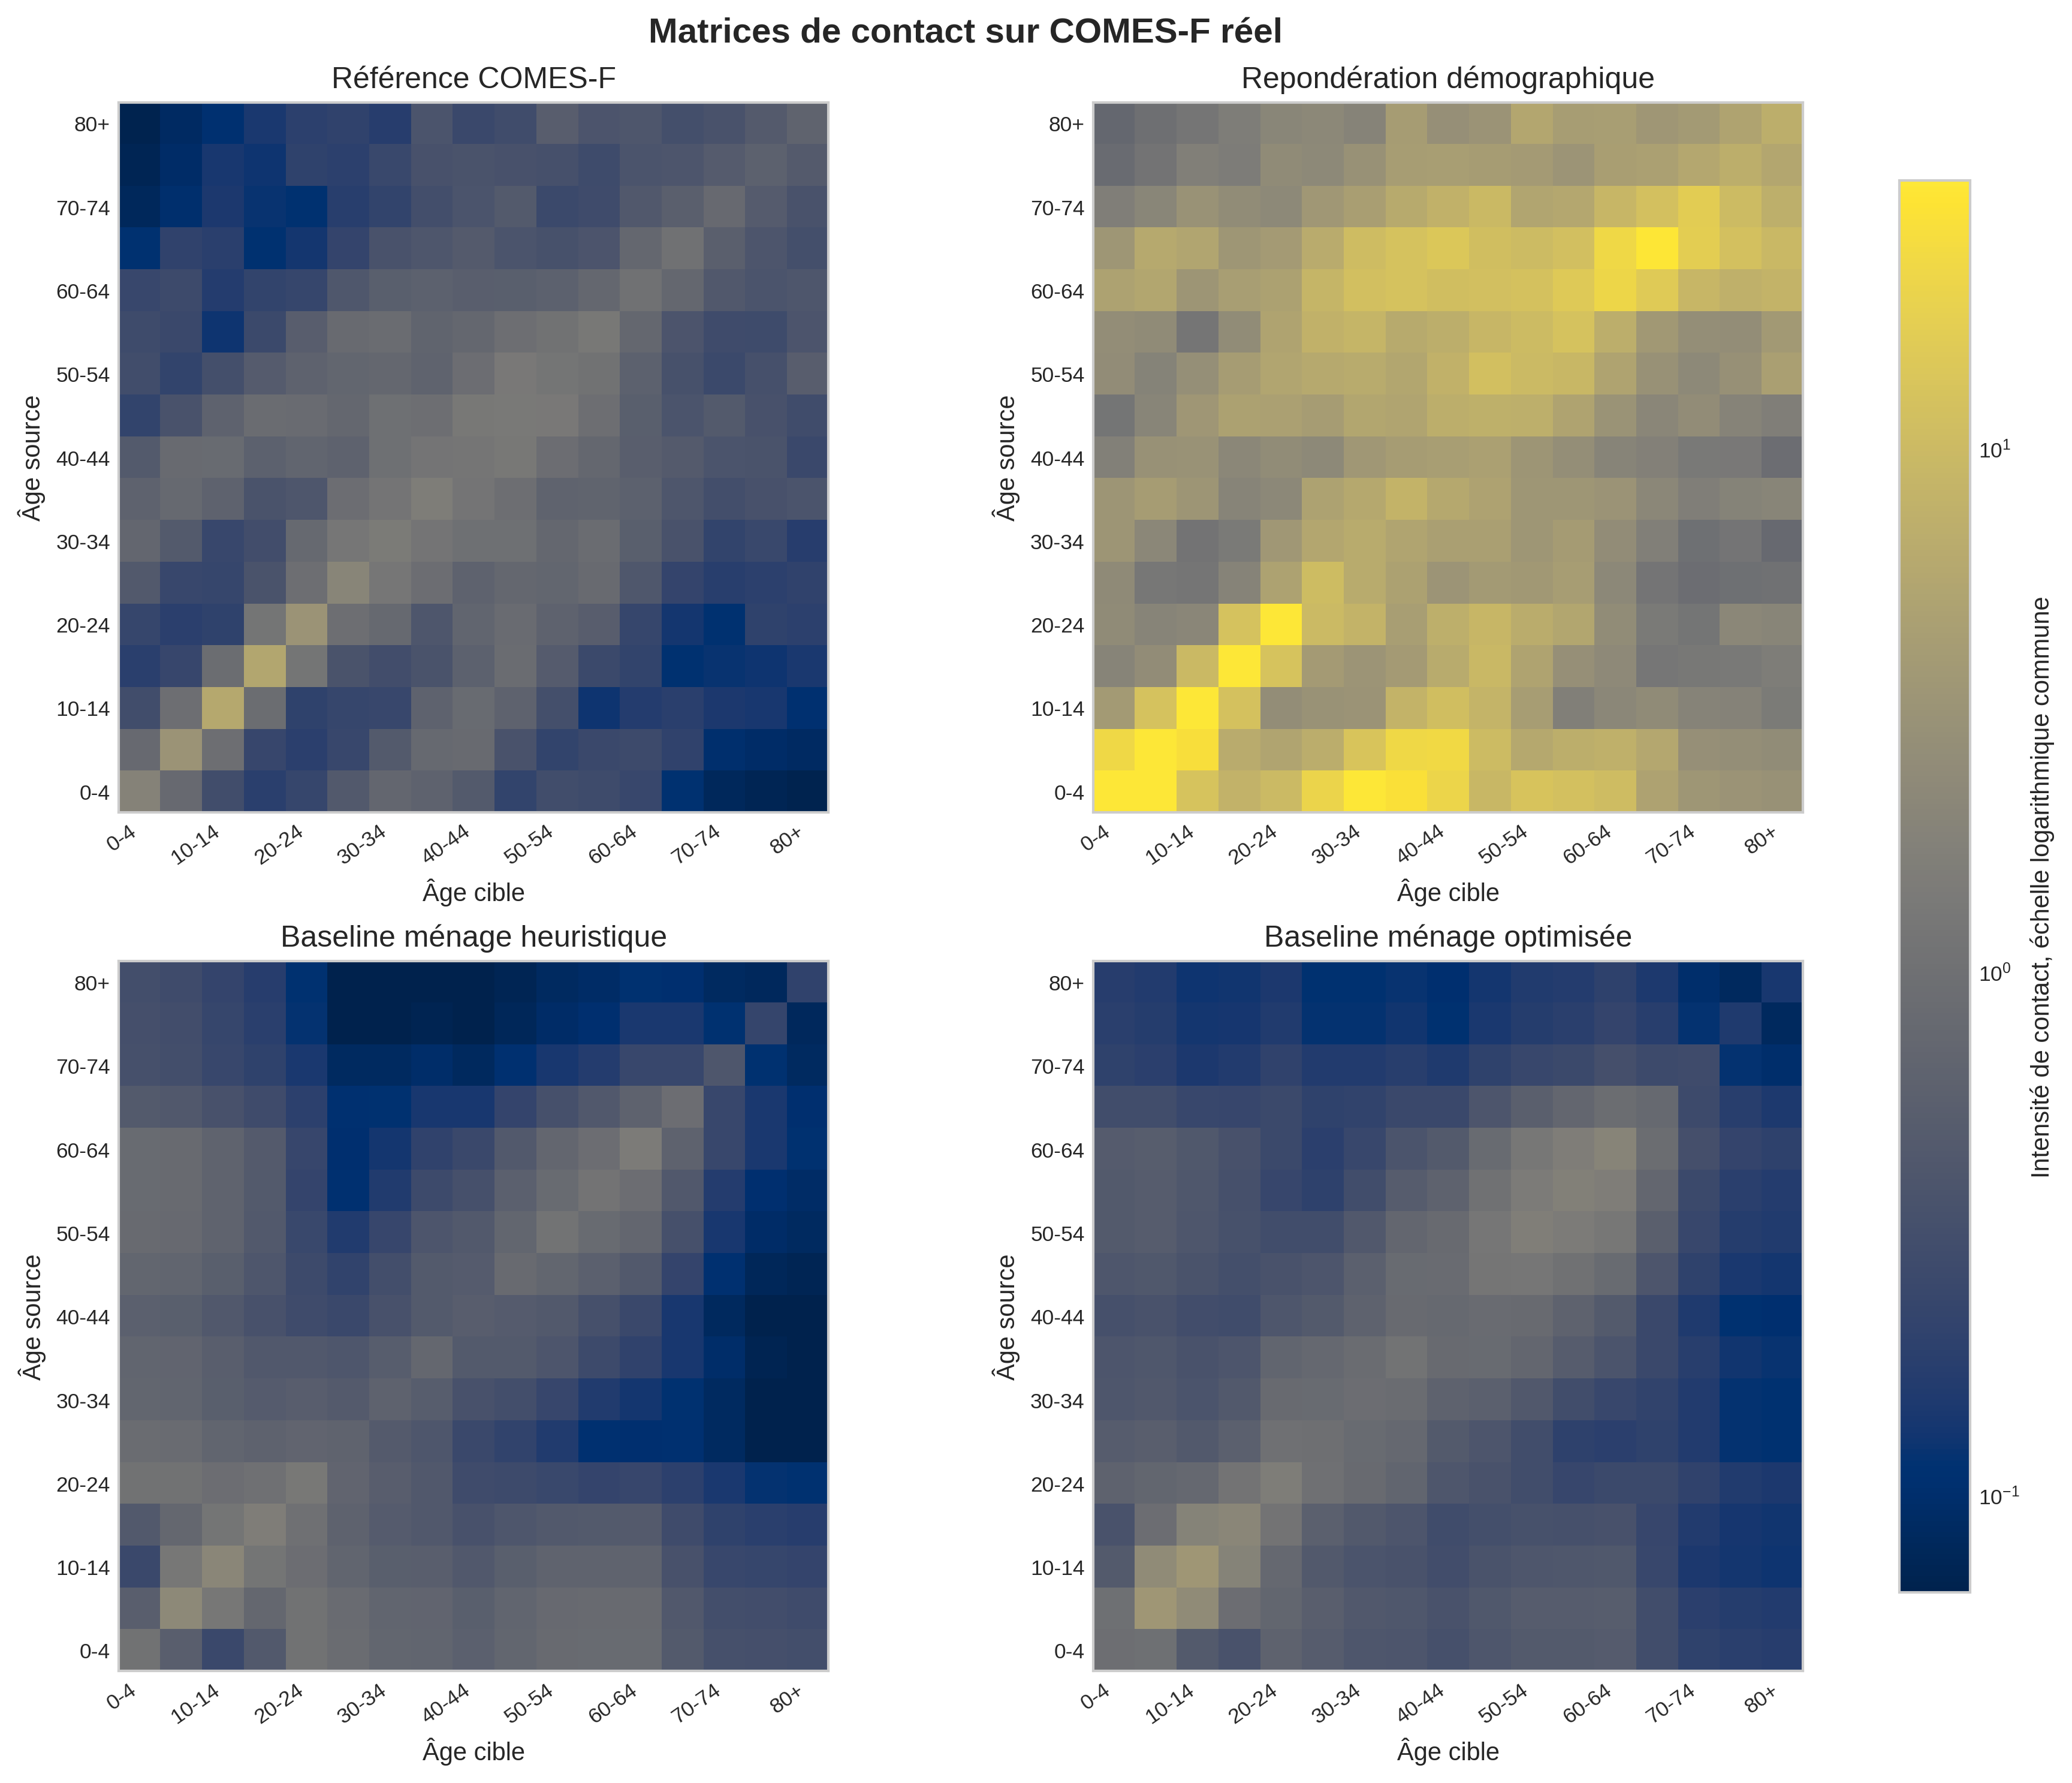
\includegraphics[width=0.98\textwidth]{figures/exp001_heatmaps.png}
    \caption{Comparaison visuelle entre la référence COMES-F, la repondération démographique, le modèle ménage heuristique et sa version optimisée. Une échelle logarithmique commune est utilisée pour conserver la comparabilité entre panneaux sans écraser les faibles intensités.}
    \label{fig:heatmaps}
\end{figure}

\begin{figure}[ht]
    \centering
    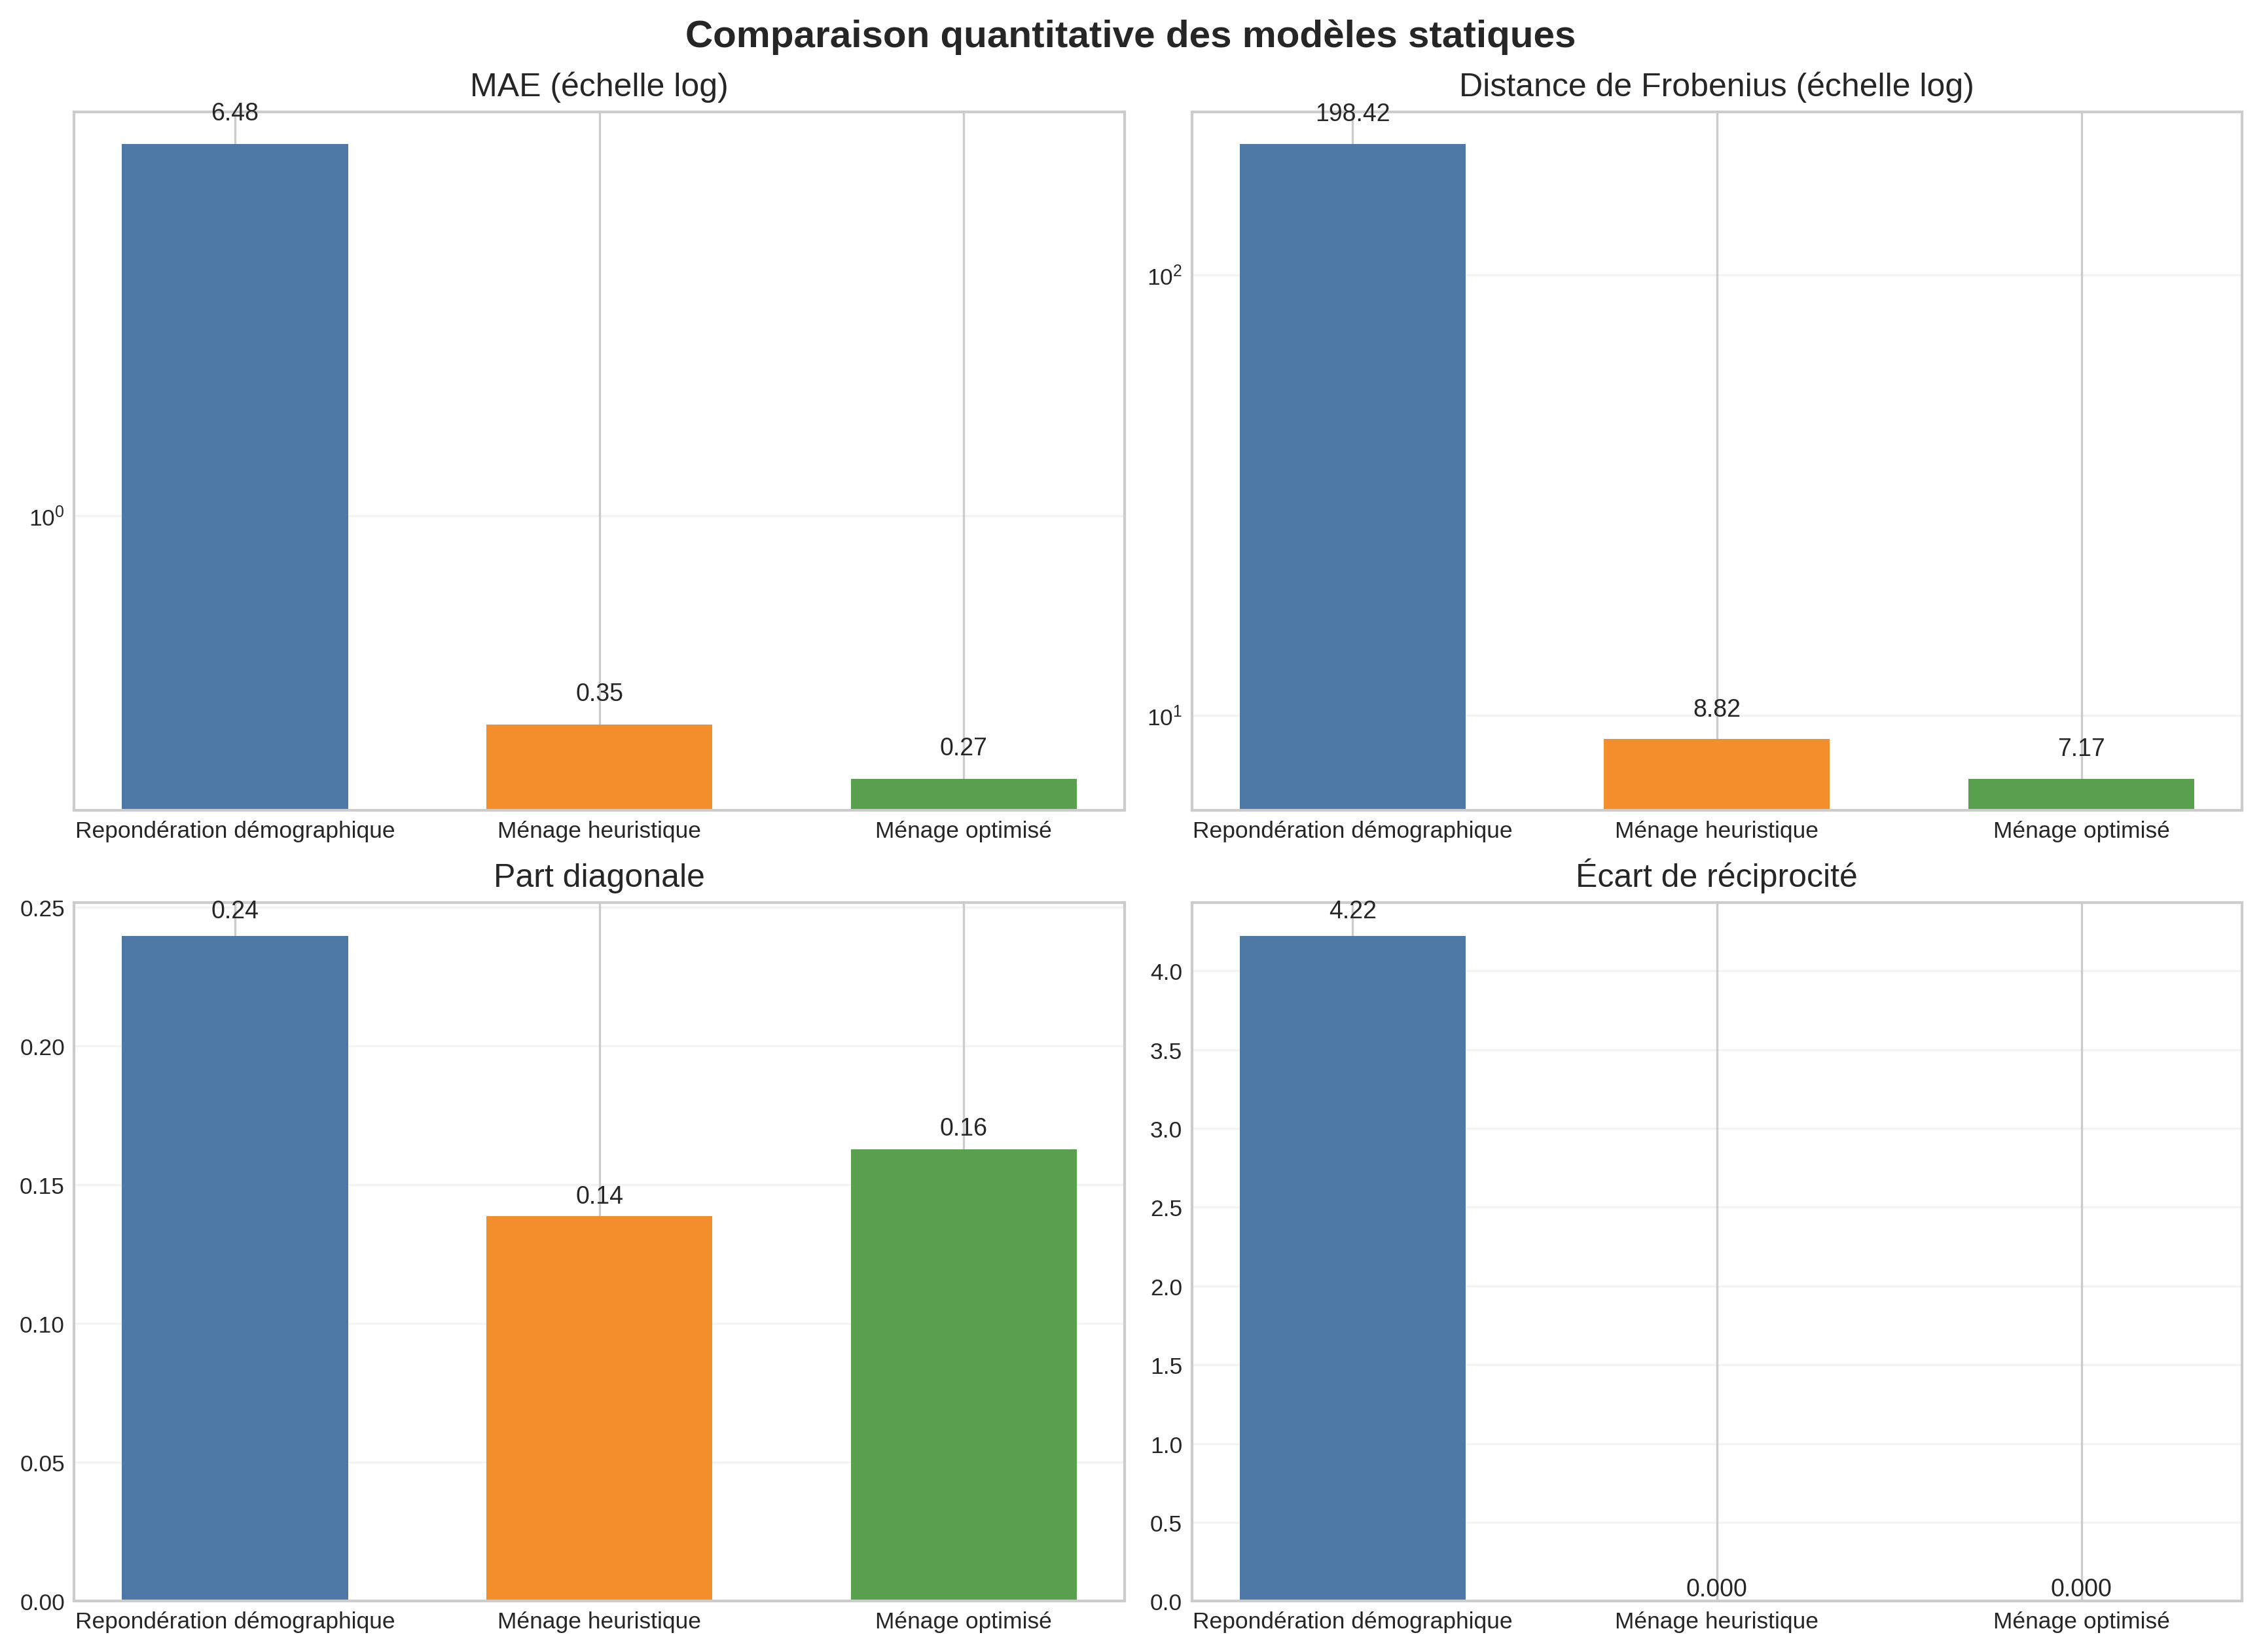
\includegraphics[width=0.98\textwidth]{figures/exp001_metrics.png}
    \caption{Comparaison des principales métriques d'erreur et de cohérence structurelle pour les trois modèles statiques.}
    \label{fig:metrics}
\end{figure}

\begin{figure}[ht]
    \centering
    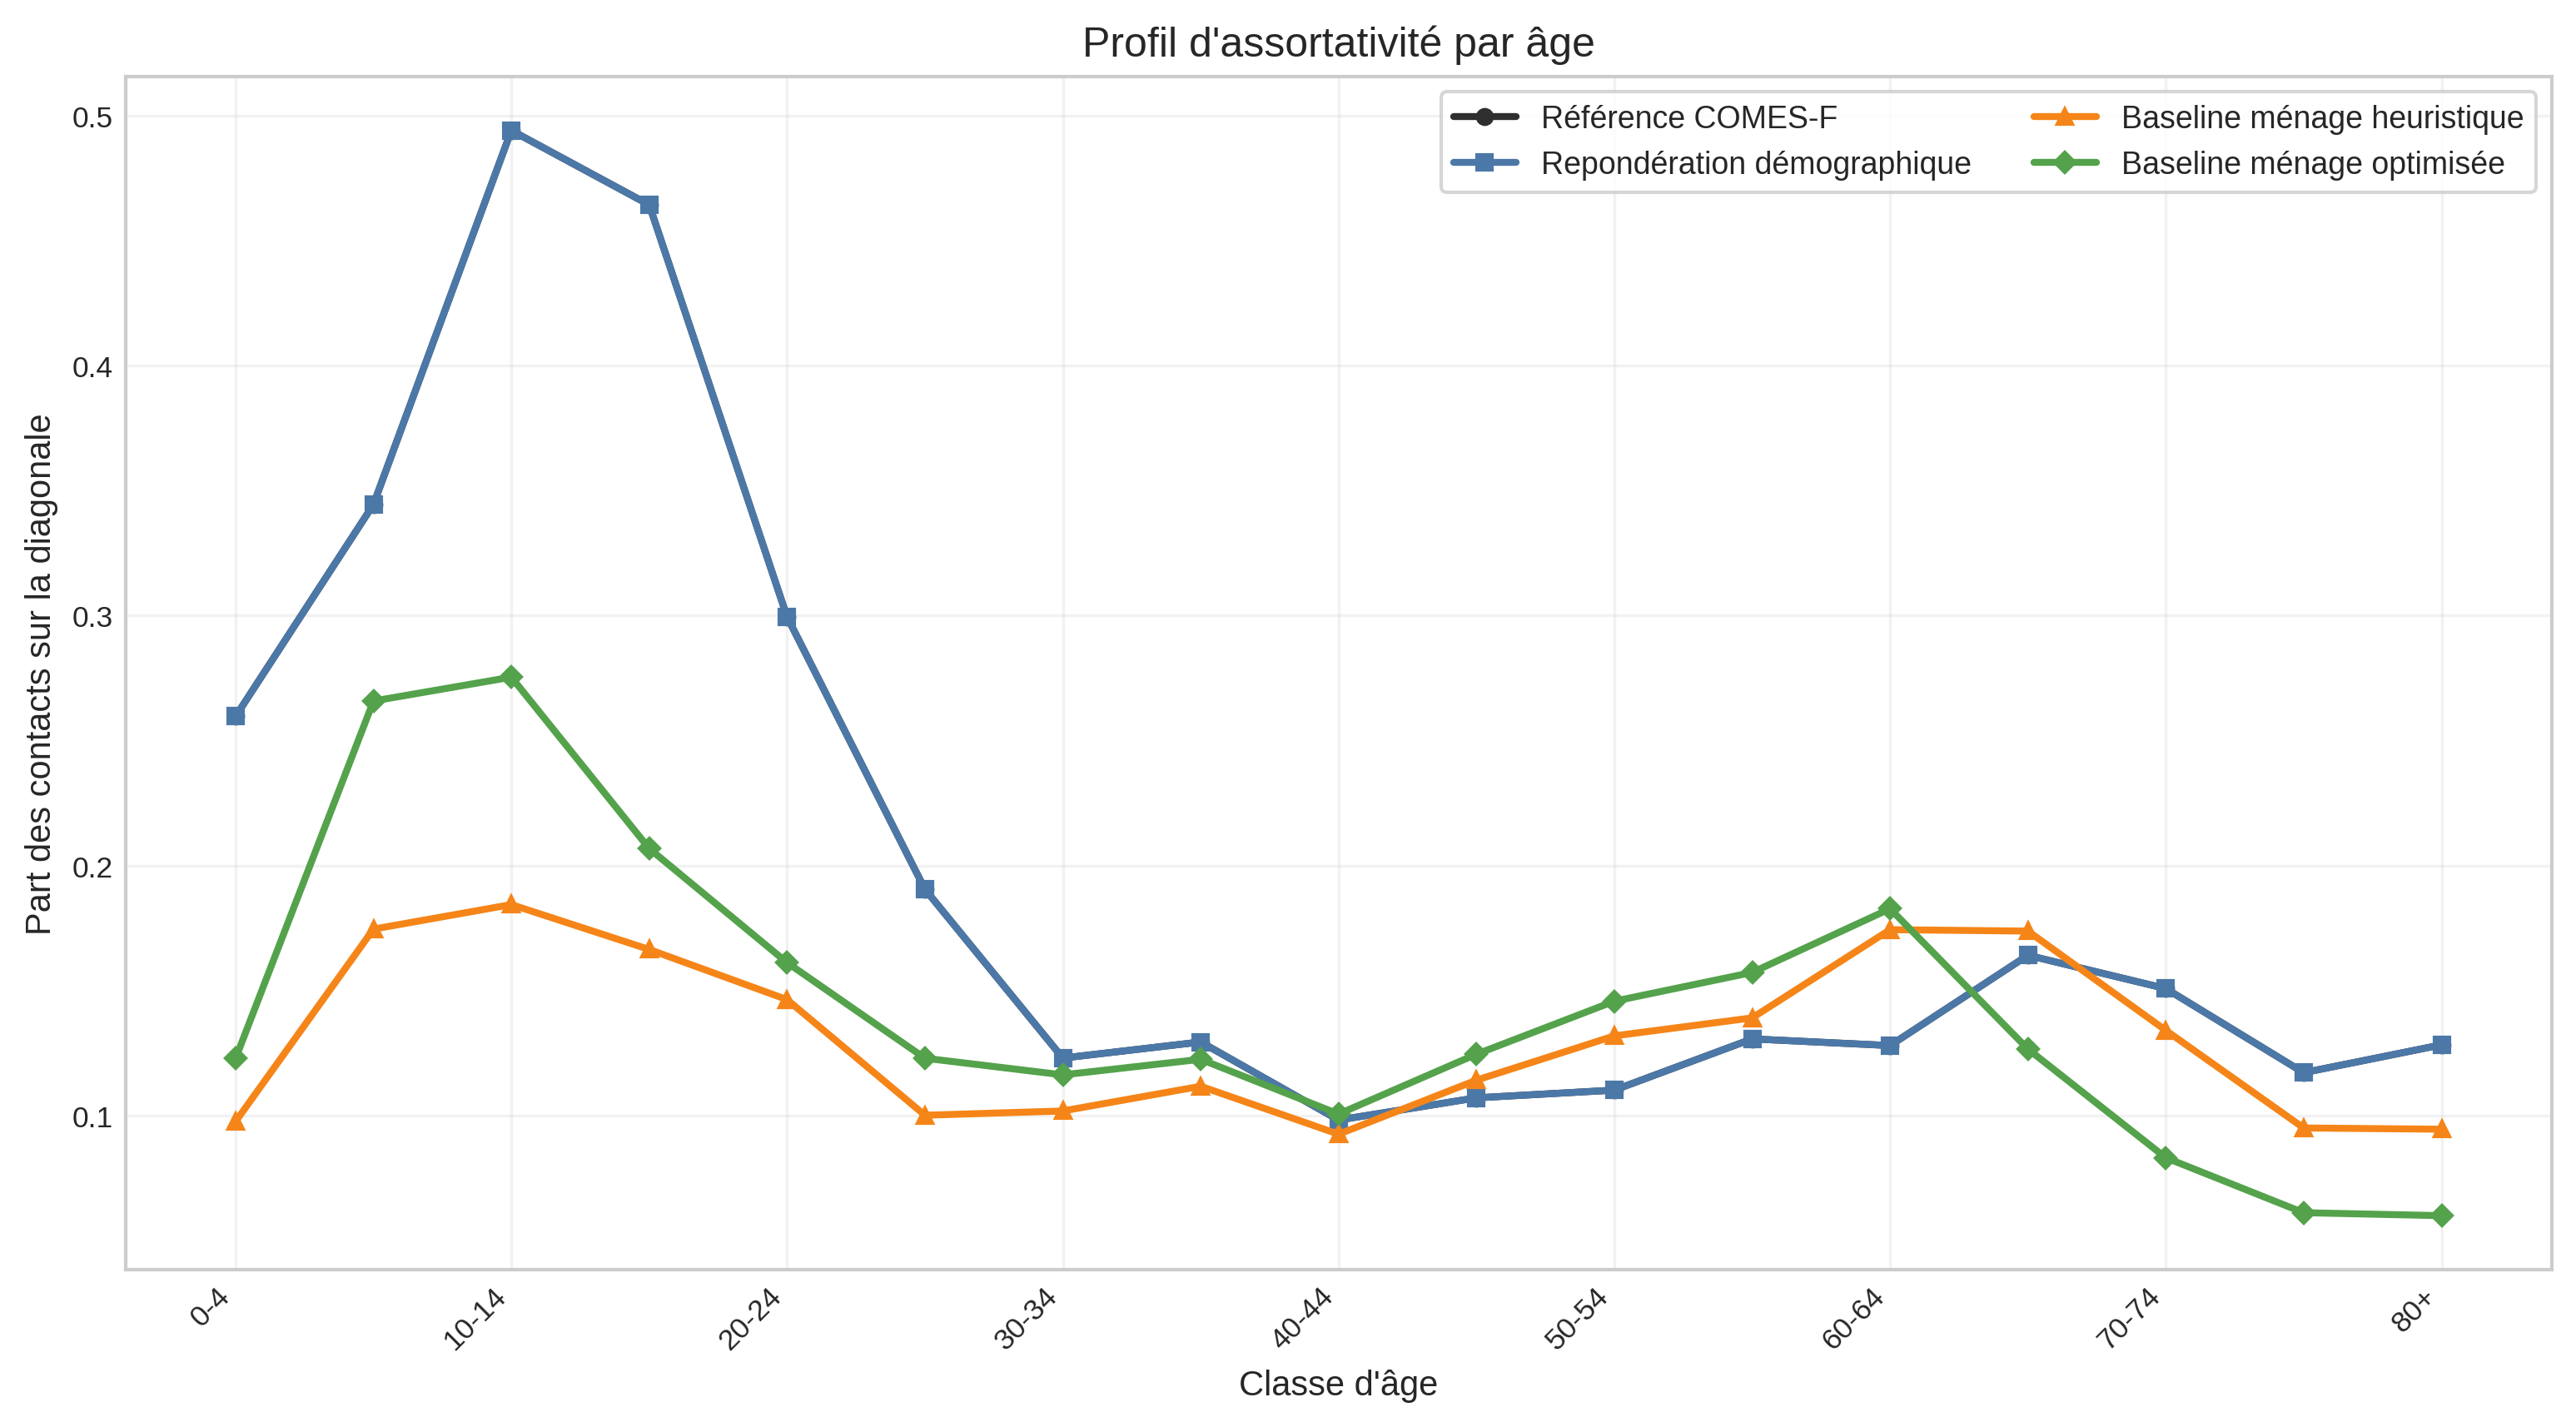
\includegraphics[width=0.80\textwidth]{figures/exp001_assortativity_profile.png}
    \caption{Profil d'assortativité par âge pour la référence empirique, la repondération démographique, le modèle ménage heuristique et sa version optimisée.}
    \label{fig:assortativity}
\end{figure}

\subsection{La couche temporelle améliore certaines séries, mais reste secondaire}
La validation temporelle nuance rapidement l'ambition du manuscrit. Une fois les fenêtres exactes de collecte SocialCov réalignées, la couche comportementale non calibrée réduit toujours la MAE de l'indice de prévention de 0,124 à 0,054 par rapport à une référence statique, avec un accord directionnel de 0,73. Sur SocialCov, en revanche, l'ajustement reste difficile : la MAE sur les changements de contacts relatifs atteint 0,265, contre 0,174 pour la référence statique, même si l'accord directionnel remonte de 0,00 à 0,40.

La calibration chronologique améliore fortement l'apprentissage, mais reste fragile hors échantillon. Pour la prévention, la MAE de test passe à 0,063, ce qui reste meilleur que la référence statique mais légèrement moins bon que la couche non calibrée. Pour les contacts SocialCov, la calibration améliore un peu la MAE de test, de 0,305 à 0,274, tout en restant nettement moins bonne que la référence statique à 0,121. L'ablation \path{remove_other_behavior} ramène la MAE de test à 0,205 sans dégrader l'accord directionnel, ce qui suggère qu'une partie de la composante communautaire absorbe encore trop brutalement les ruptures de politique publique.

\begin{table}[ht]
    \centering
    \small
    \caption{Synthèse des métriques temporelles après réalignement SocialCov et calibration. Toutes les colonnes sont des scores sans unité compris entre 0 et 1, sauf la MAE qui reste exprimée sur l'échelle normalisée des séries.}
    \begin{tabularx}{\linewidth}{>{\raggedright\arraybackslash}X r r r}
        \toprule
        Série et modèle & MAE & Accord directionnel & Précision du pic \\
        \midrule
        Prévention, comportemental non calibré & 0{,}054 & 0{,}73 & 0{,}50 \\
        Prévention, statique & 0{,}124 & 0{,}00 & 0{,}50 \\
        Contacts, comportemental non calibré & 0{,}265 & 0{,}40 & 1{,}00 \\
        Contacts, statique & 0{,}174 & 0{,}00 & 0{,}20 \\
        Prévention test, calibré & 0{,}063 & 0{,}50 & 0{,}20 \\
        Contacts test, calibré & 0{,}274 & 1{,}00 & 1{,}00 \\
        \bottomrule
    \end{tabularx}
\end{table}

Les figures \ref{fig:exp003-prevention} et \ref{fig:exp003-contacts} résument cette dissymétrie : le signal temporel est utile pour documenter des comportements agrégés, mais il ne suffit pas à porter la contribution principale du papier. Il reste un étage intermédiaire utile, pas le centre de gravité du manuscrit.

\begin{figure}[ht]
    \centering
    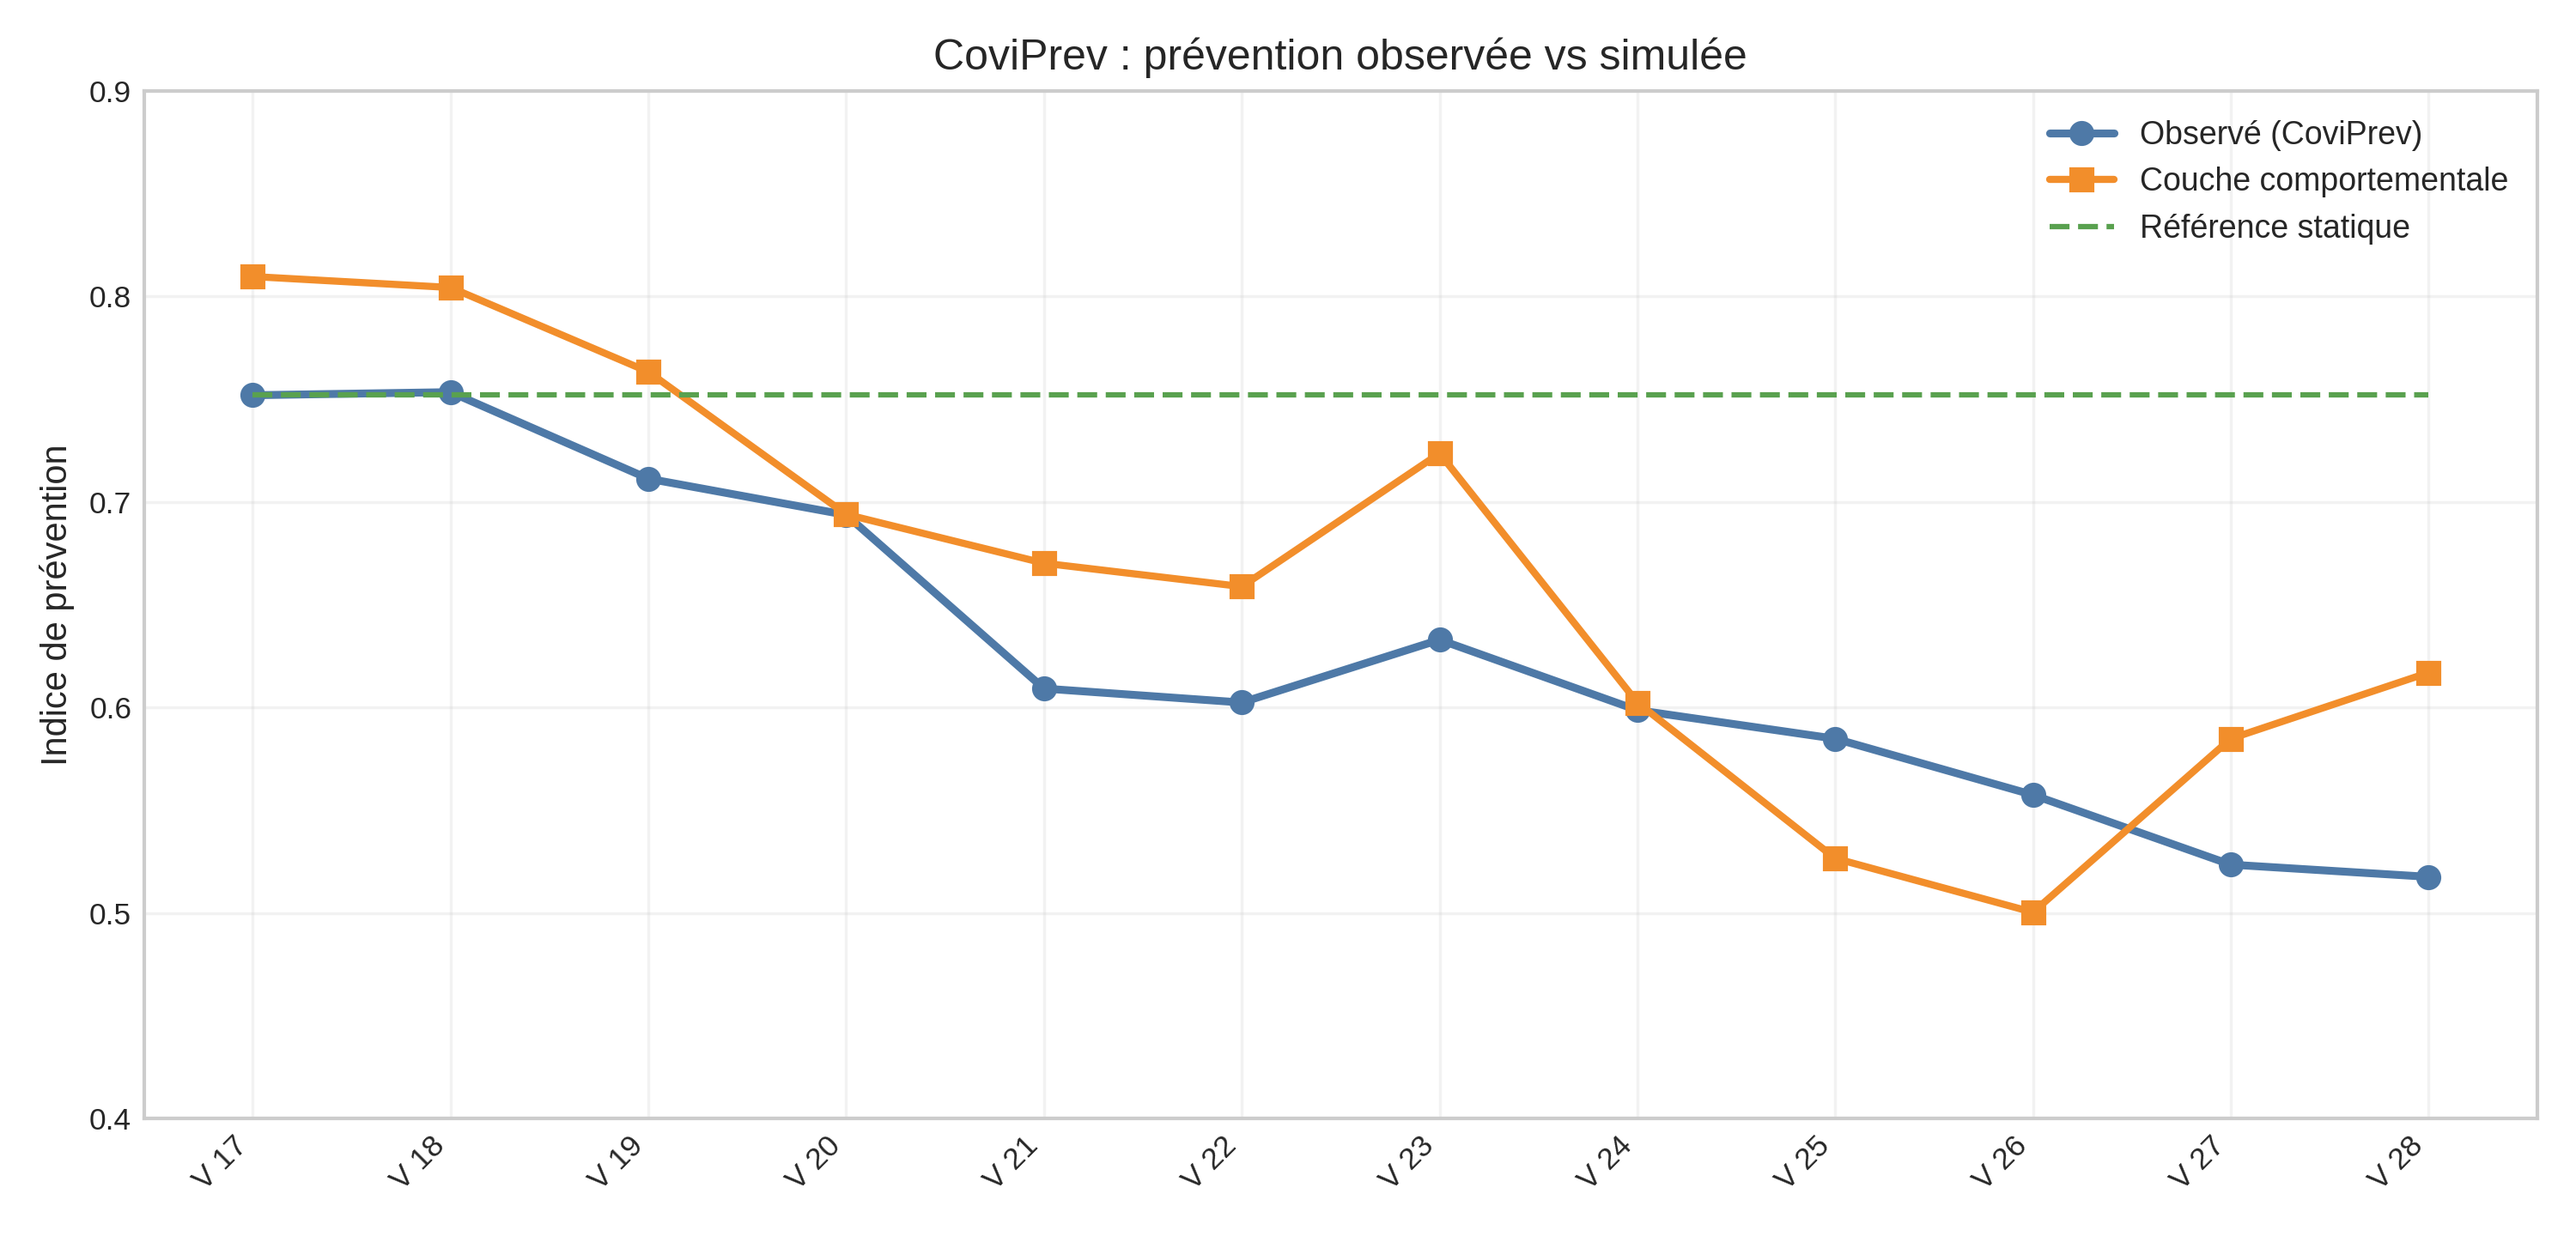
\includegraphics[width=0.92\textwidth]{figures/exp003_preventive_behavior_timeseries.png}
    \caption{Indice de prévention observé dans CoviPrev et simulé par la couche comportementale.}
    \label{fig:exp003-prevention}
\end{figure}

\begin{figure}[ht]
    \centering
    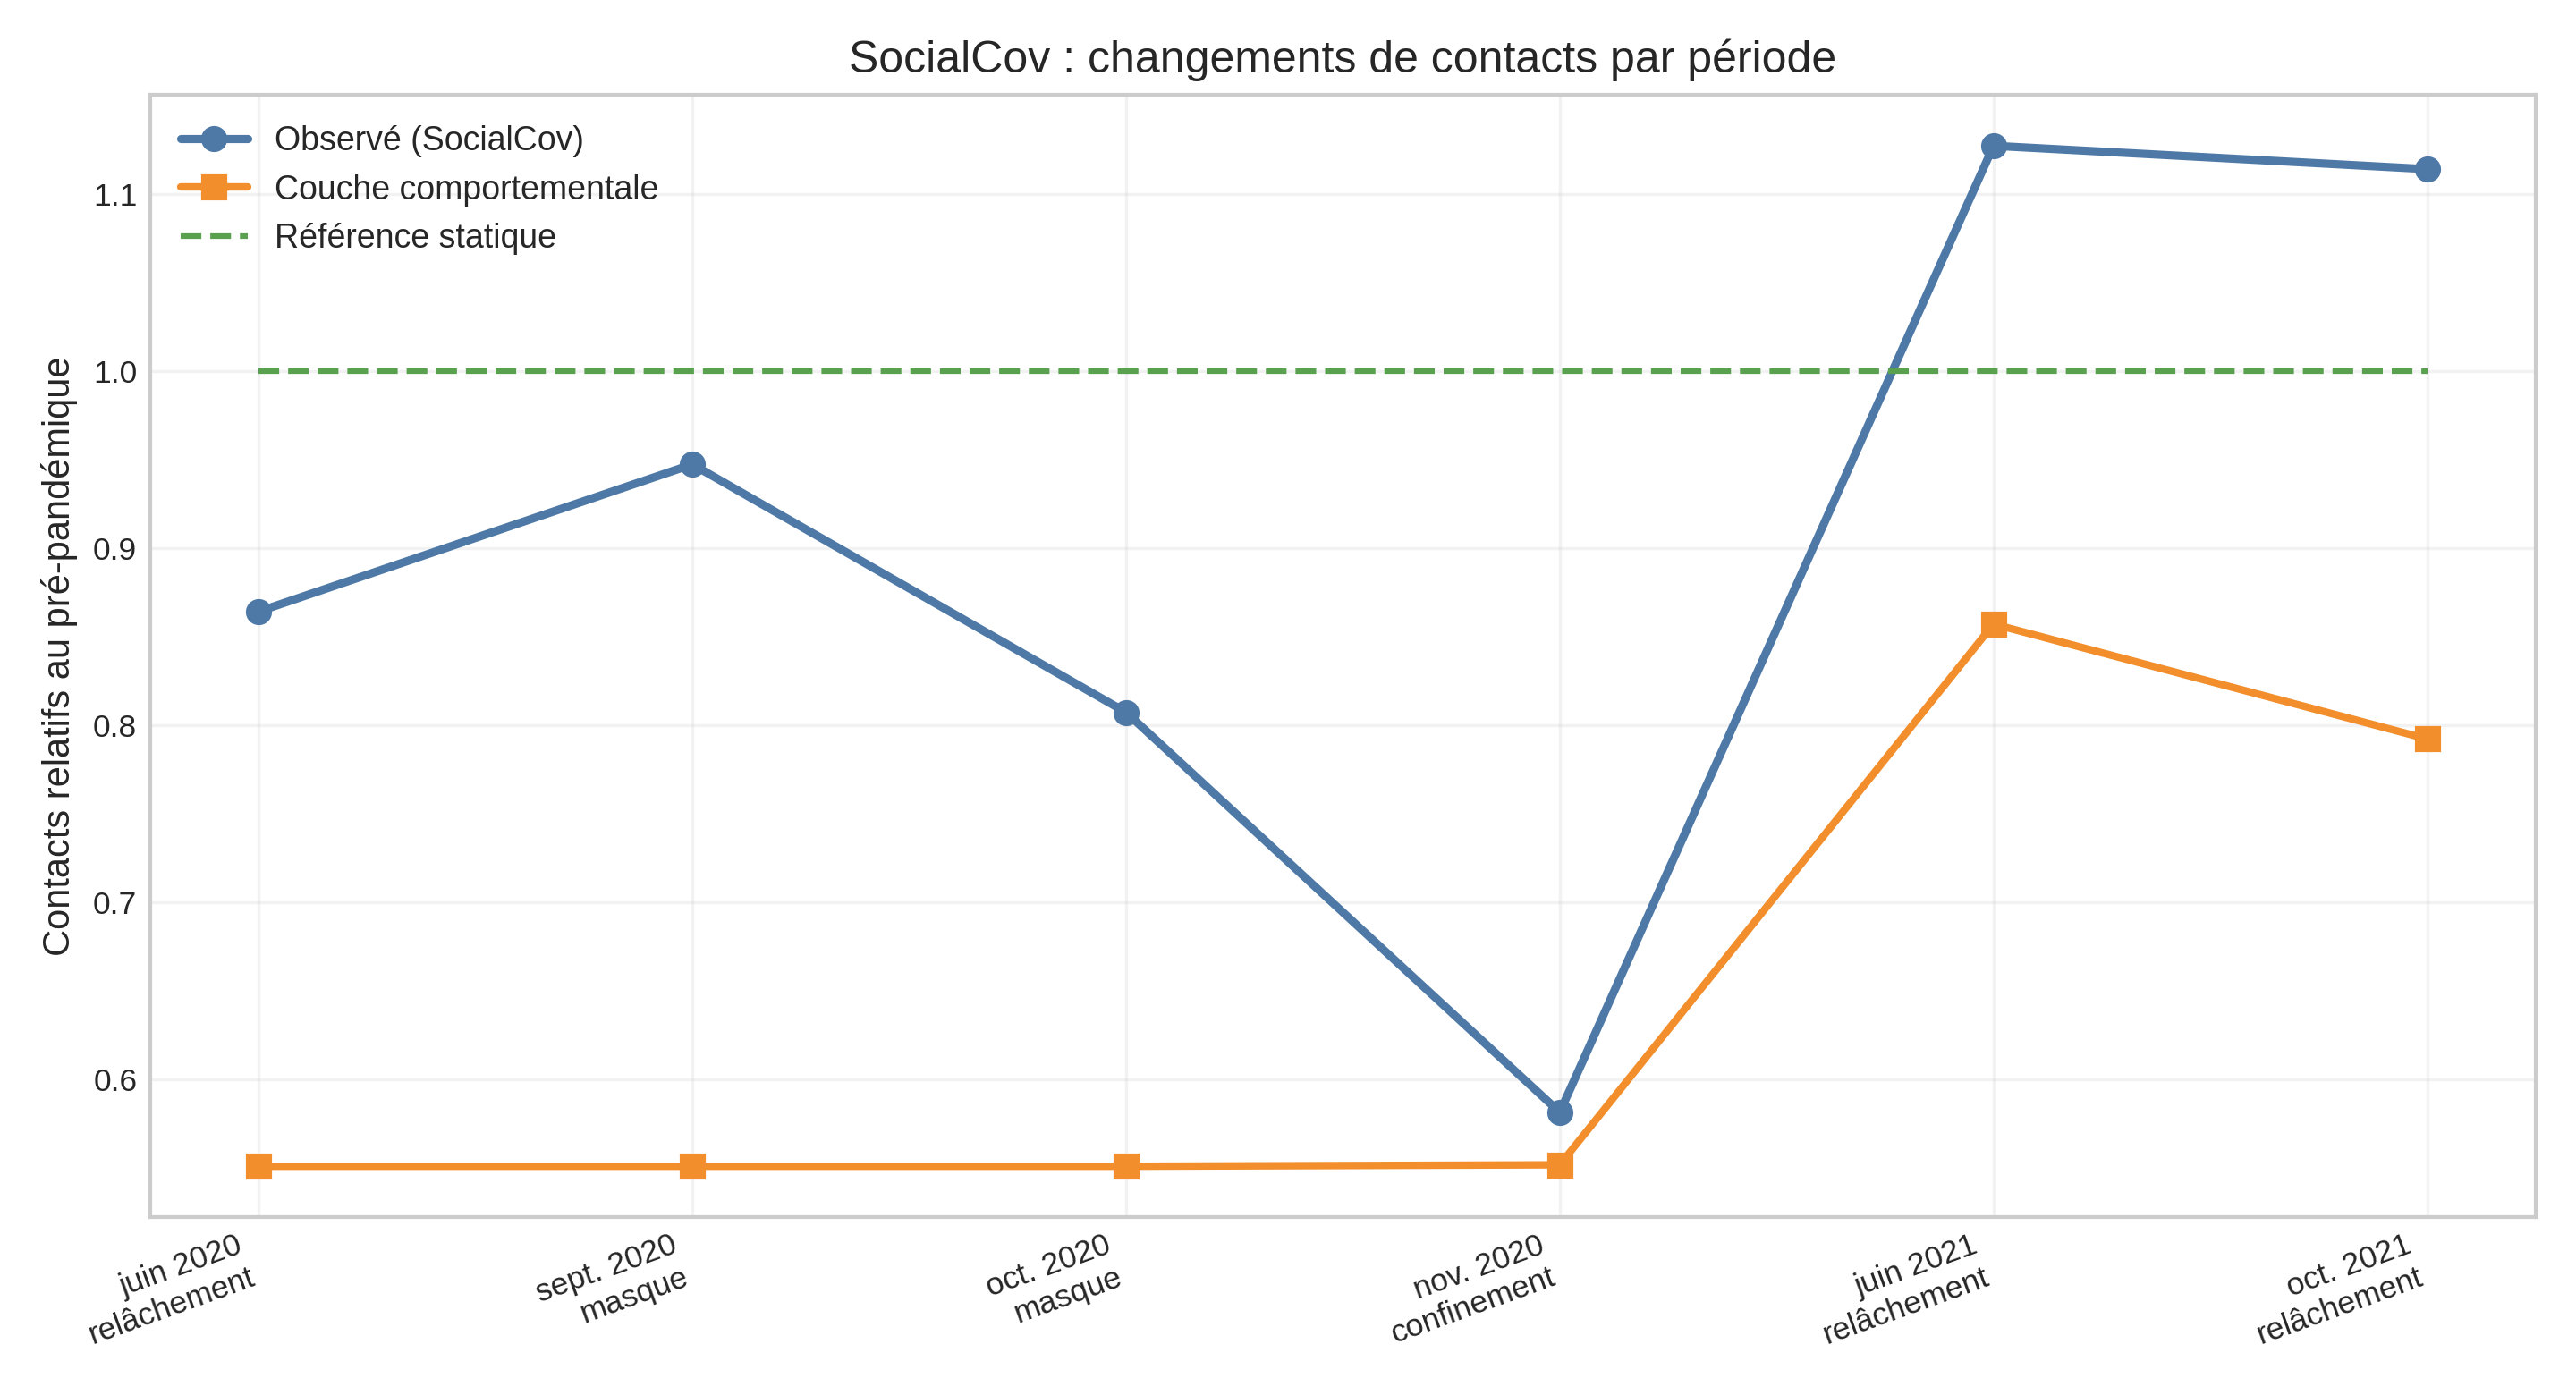
\includegraphics[width=0.88\textwidth]{figures/exp003_contact_changes_periods.png}
    \caption{Changements de contacts relatifs observés dans SocialCov et simulés par la couche comportementale.}
    \label{fig:exp003-contacts}
\end{figure}

\subsection{Premier résultat central : la couche LLM fait émerger une hétérogénéité sociale lisible}
L'expérience \texttt{exp006\_llm\_agents} constitue le premier résultat central du papier. Contrairement aux versions intermédiaires du pipeline, l'exécution retenue ici repose sur des appels réels à Claude Sonnet 4.6, avec 18 profils, six régimes de politique publique et 108 couples profil-régime archivés. Le premier résultat est un gradient temporel net et cohérent avec l'histoire sanitaire : la réduction moyenne de mobilité simulée passe de 0,09 en pré-pandémie à 0,71 lors du premier confinement, avant de redescendre à 0,40 au déconfinement puis de remonter à 0,50 pendant la seconde vague, 0,61 sous couvre-feu et 0,41 pendant le passe sanitaire. L'adhésion moyenne au masque suit elle aussi une trajectoire plausible.

\begin{table}[ht]
    \centering
    \small
    \caption{Résumé des sorties LLM agrégées par régime sanitaire pour la première campagne \texttt{exp006}. Les trois colonnes numériques sont des scores bornés entre 0 et 1.}
    \begin{tabularx}{\linewidth}{>{\raggedright\arraybackslash}X r r r}
        \toprule
        Régime & Mobilité LLM & Mobilité observée & Masque LLM \\
        \midrule
        Pré-pandémie & 0{,}09 & 0{,}05 & 0{,}04 \\
        Premier confinement & 0{,}71 & 0{,}63 & 0{,}56 \\
        Déconfinement & 0{,}40 & 0{,}18 & 0{,}69 \\
        Deuxième vague & 0{,}50 & 0{,}29 & 0{,}79 \\
        Couvre-feu & 0{,}61 & 0{,}27 & 0{,}80 \\
        Passe sanitaire & 0{,}41 & 0{,}06 & 0{,}74 \\
        \bottomrule
    \end{tabularx}
\end{table}

Pris isolément, ce premier bloc LLM reste imparfait. Sur six régimes seulement, la corrélation entre réduction de mobilité simulée et mobilité observée vaut 0,826, avec une MAE de 0,206. Ce n'est pas une calibration fine. En revanche, c'est déjà un résultat utile pour les SHS et pour l'épidémiologie appliquée : le modèle restitue correctement l'ordre général des régimes sanitaires et rend visible une différenciation sociale de la capacité d'ajustement.

Le résultat le plus intéressant concerne en effet la hiérarchie de réactivité entre profils. La différence entre le profil \emph{cadre 35-49 en couple avec enfants} et le profil \emph{agriculteur 50-64 en couple} est nette et socialement interprétable. Les profils cadres cumulent télétravail, flexibilité numérique et confiance plus élevée dans les mesures. Les profils agricoles ou ouvriers restent davantage contraints par le présentiel, la continuité de l'activité et une marge d'ajustement moindre. Les figures \ref{fig:exp006-mobility}, \ref{fig:exp006-ranking} et \ref{fig:exp006-bias} synthétisent ce double résultat : bon ordonnancement des régimes, puis différenciation sociale explicite.

\begin{figure}[ht]
    \centering
    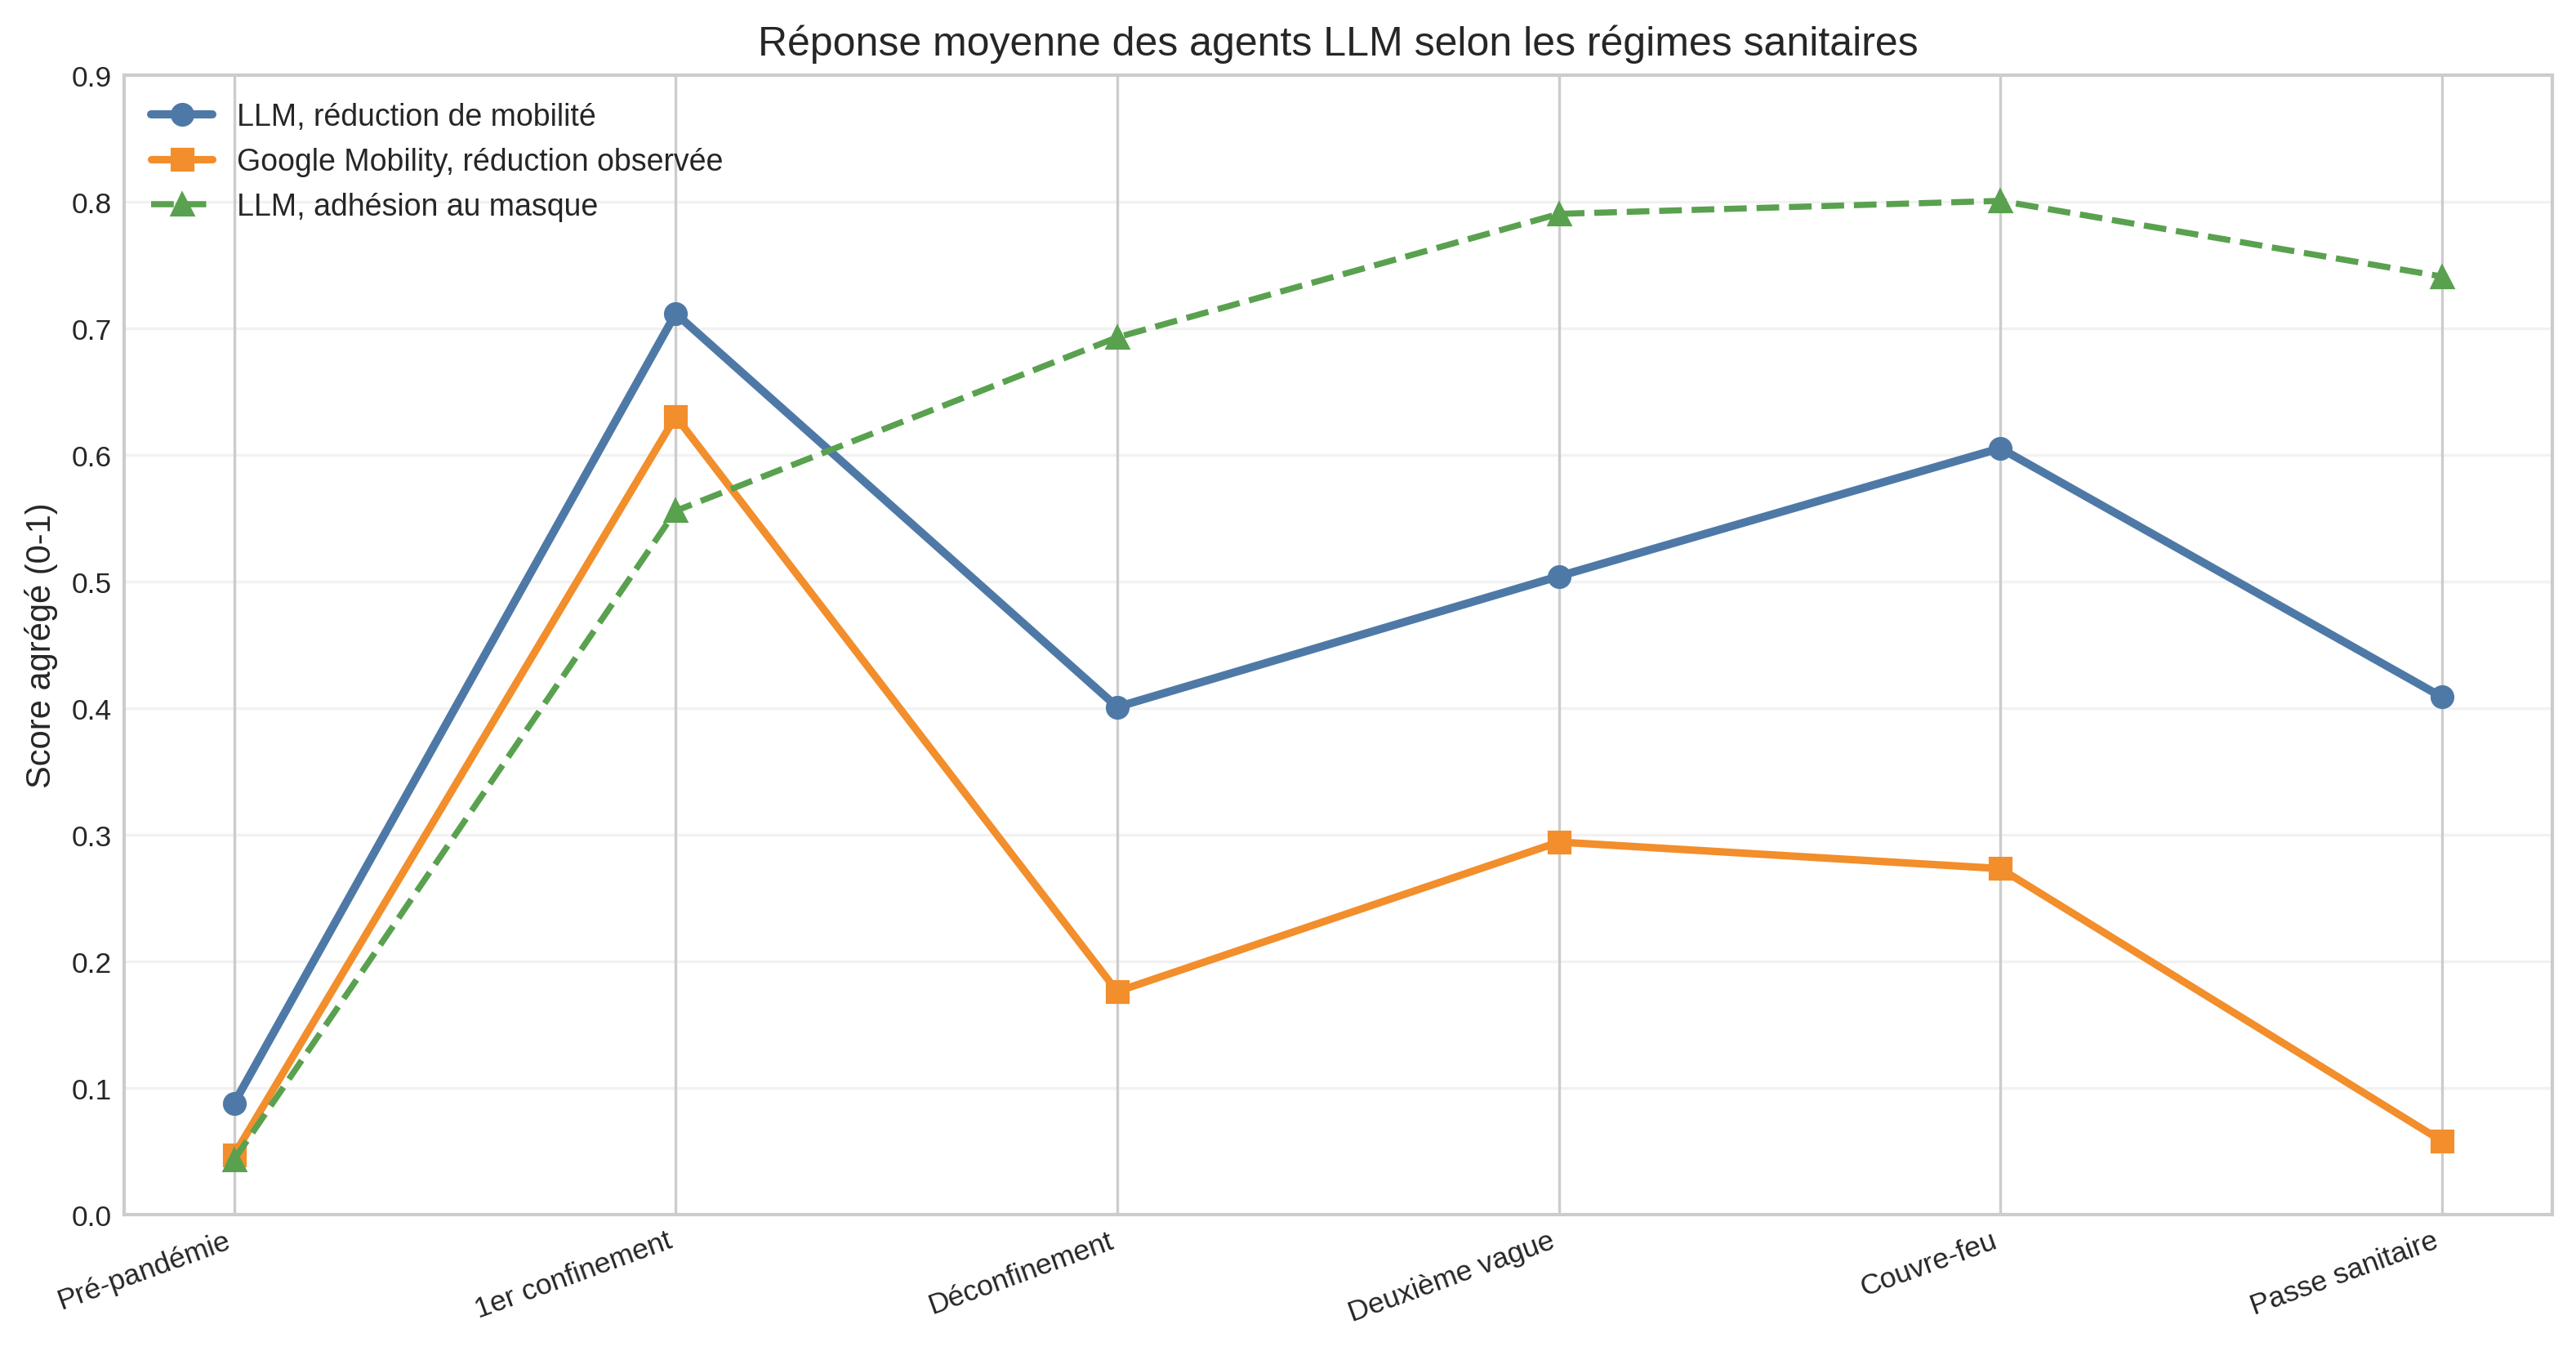
\includegraphics[width=0.92\textwidth]{figures/exp006_llm_vs_observed_mobility_by_policy.png}
    \caption{Réduction de mobilité agrégée des agents LLM, comparée à l'indice observé de Google Mobility, avec rappel de l'adhésion moyenne au masque.}
    \label{fig:exp006-mobility}
\end{figure}

\begin{figure}[ht]
    \centering
    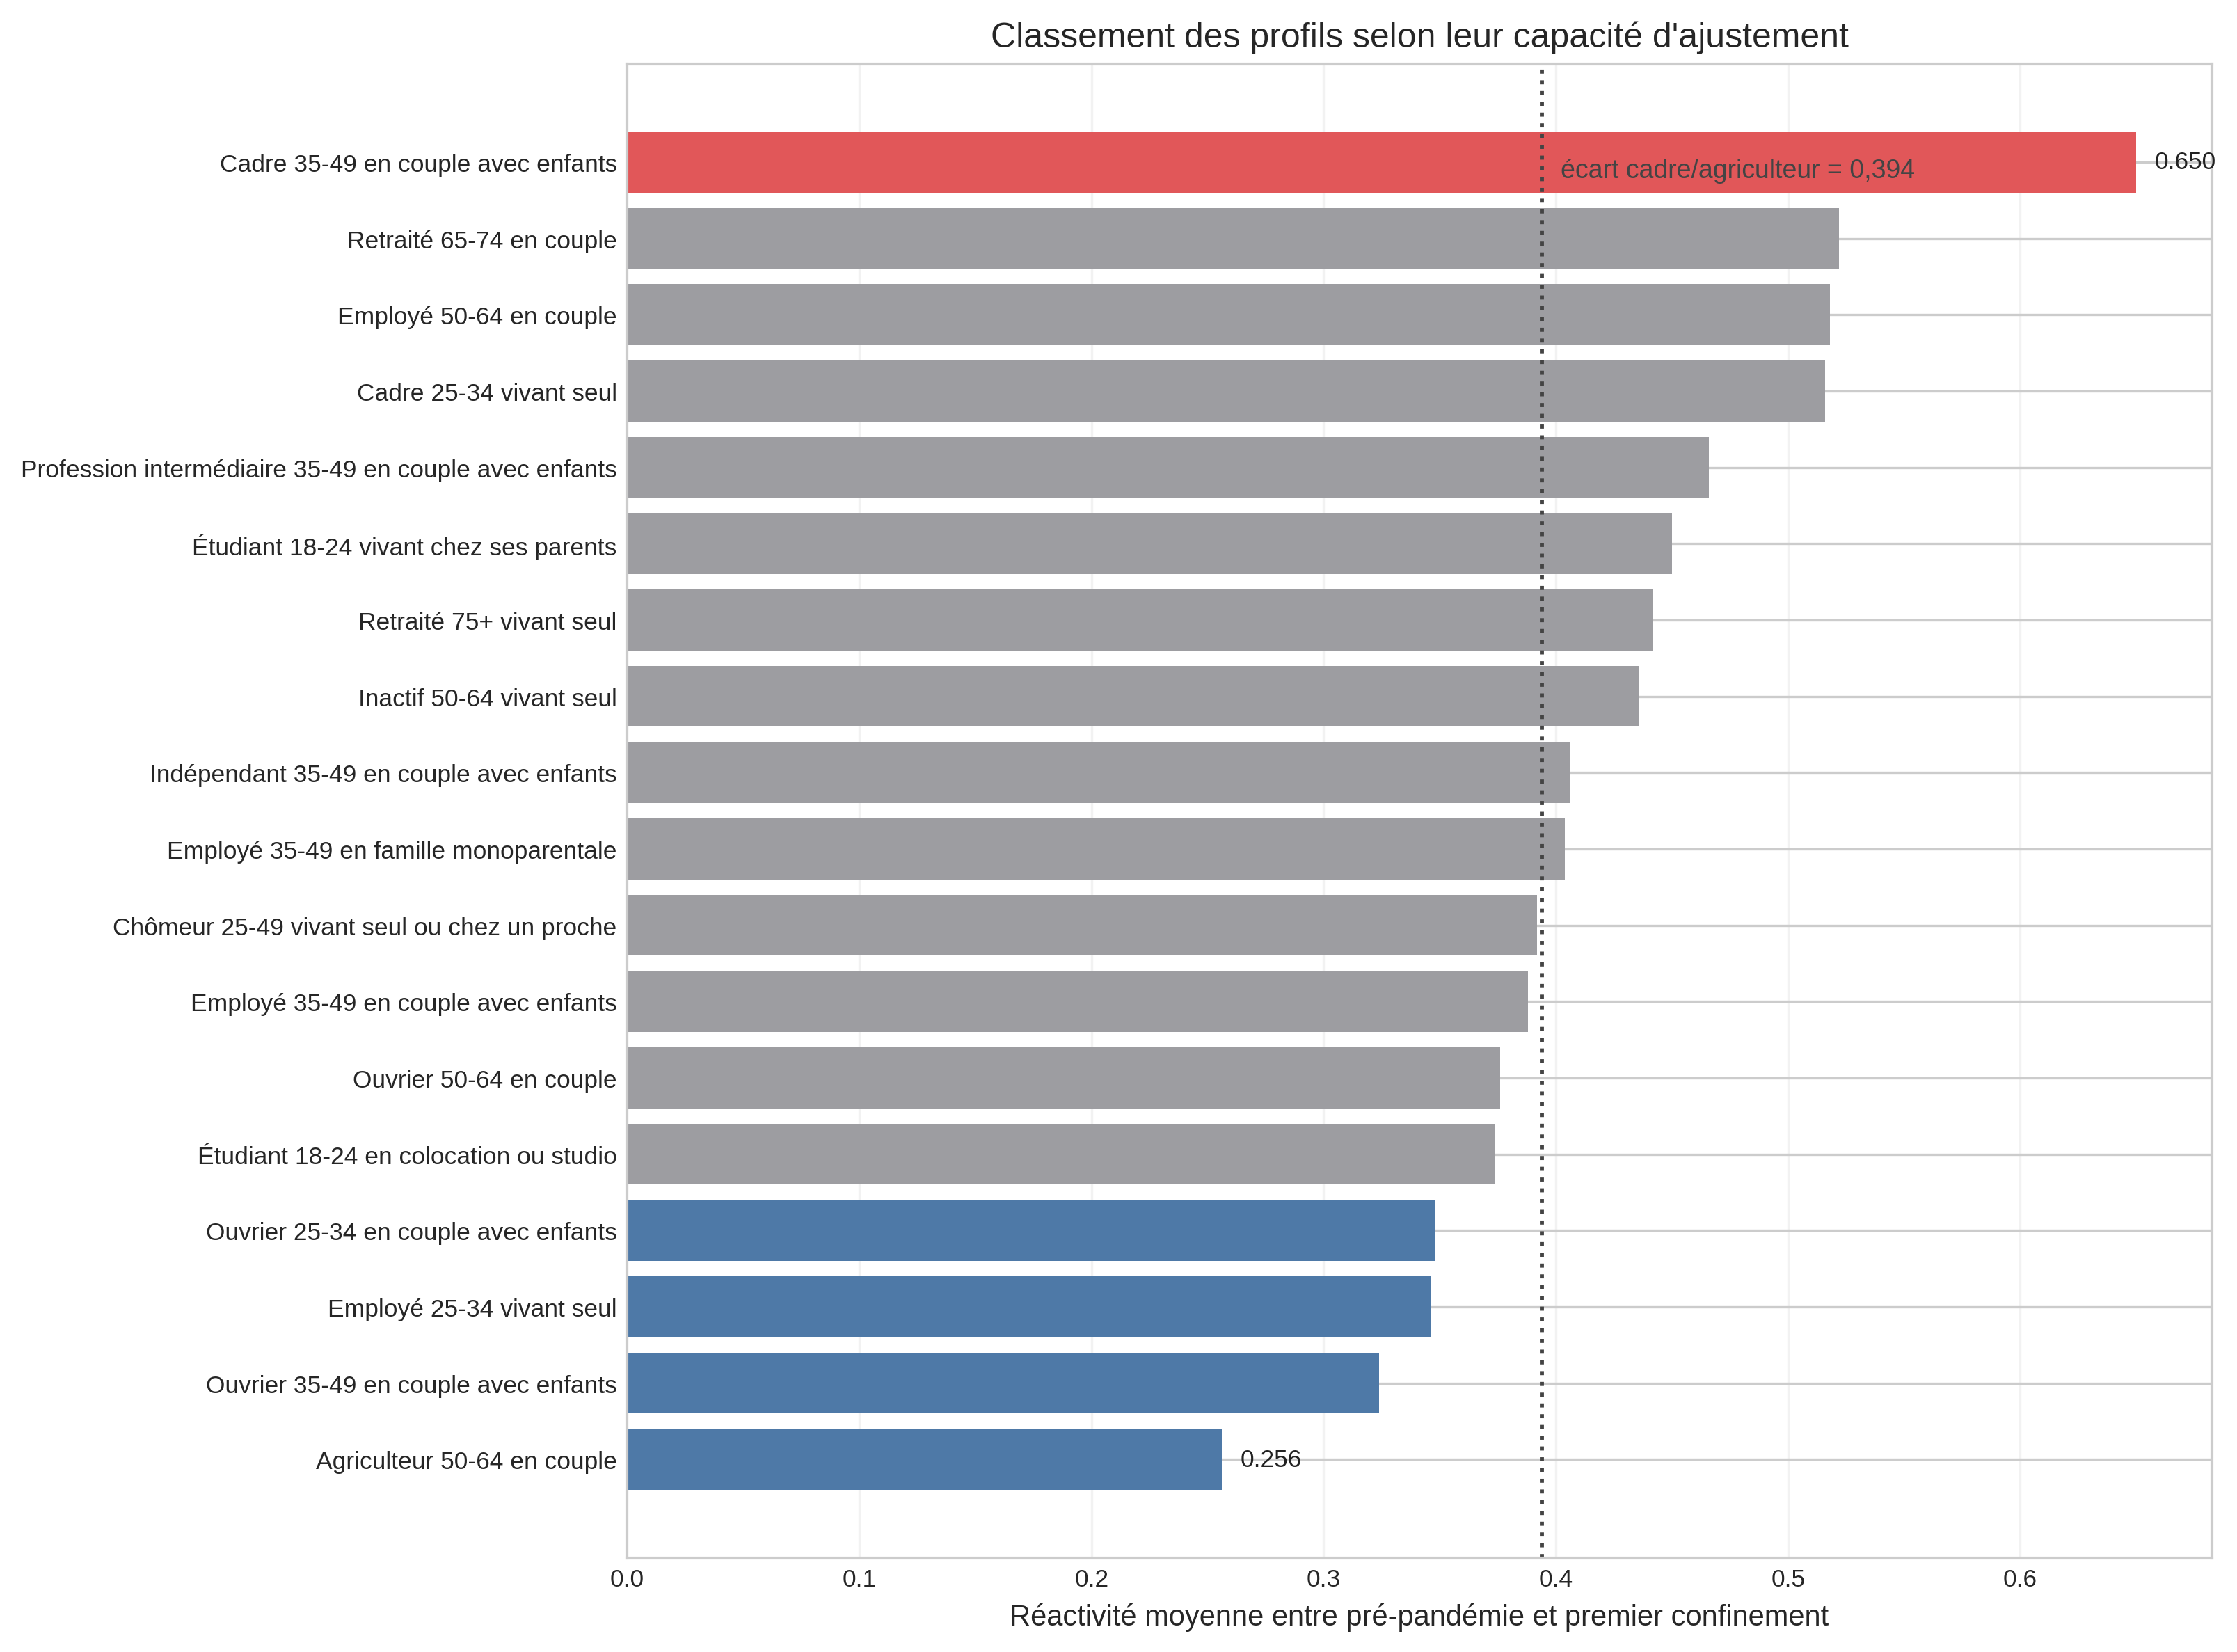
\includegraphics[width=0.92\textwidth]{figures/exp006_profile_responsiveness_ranking.png}
    \caption{Classement des 18 profils selon leur réactivité moyenne entre la pré-pandémie et le premier confinement.}
    \label{fig:exp006-ranking}
\end{figure}

\begin{figure}[ht]
    \centering
    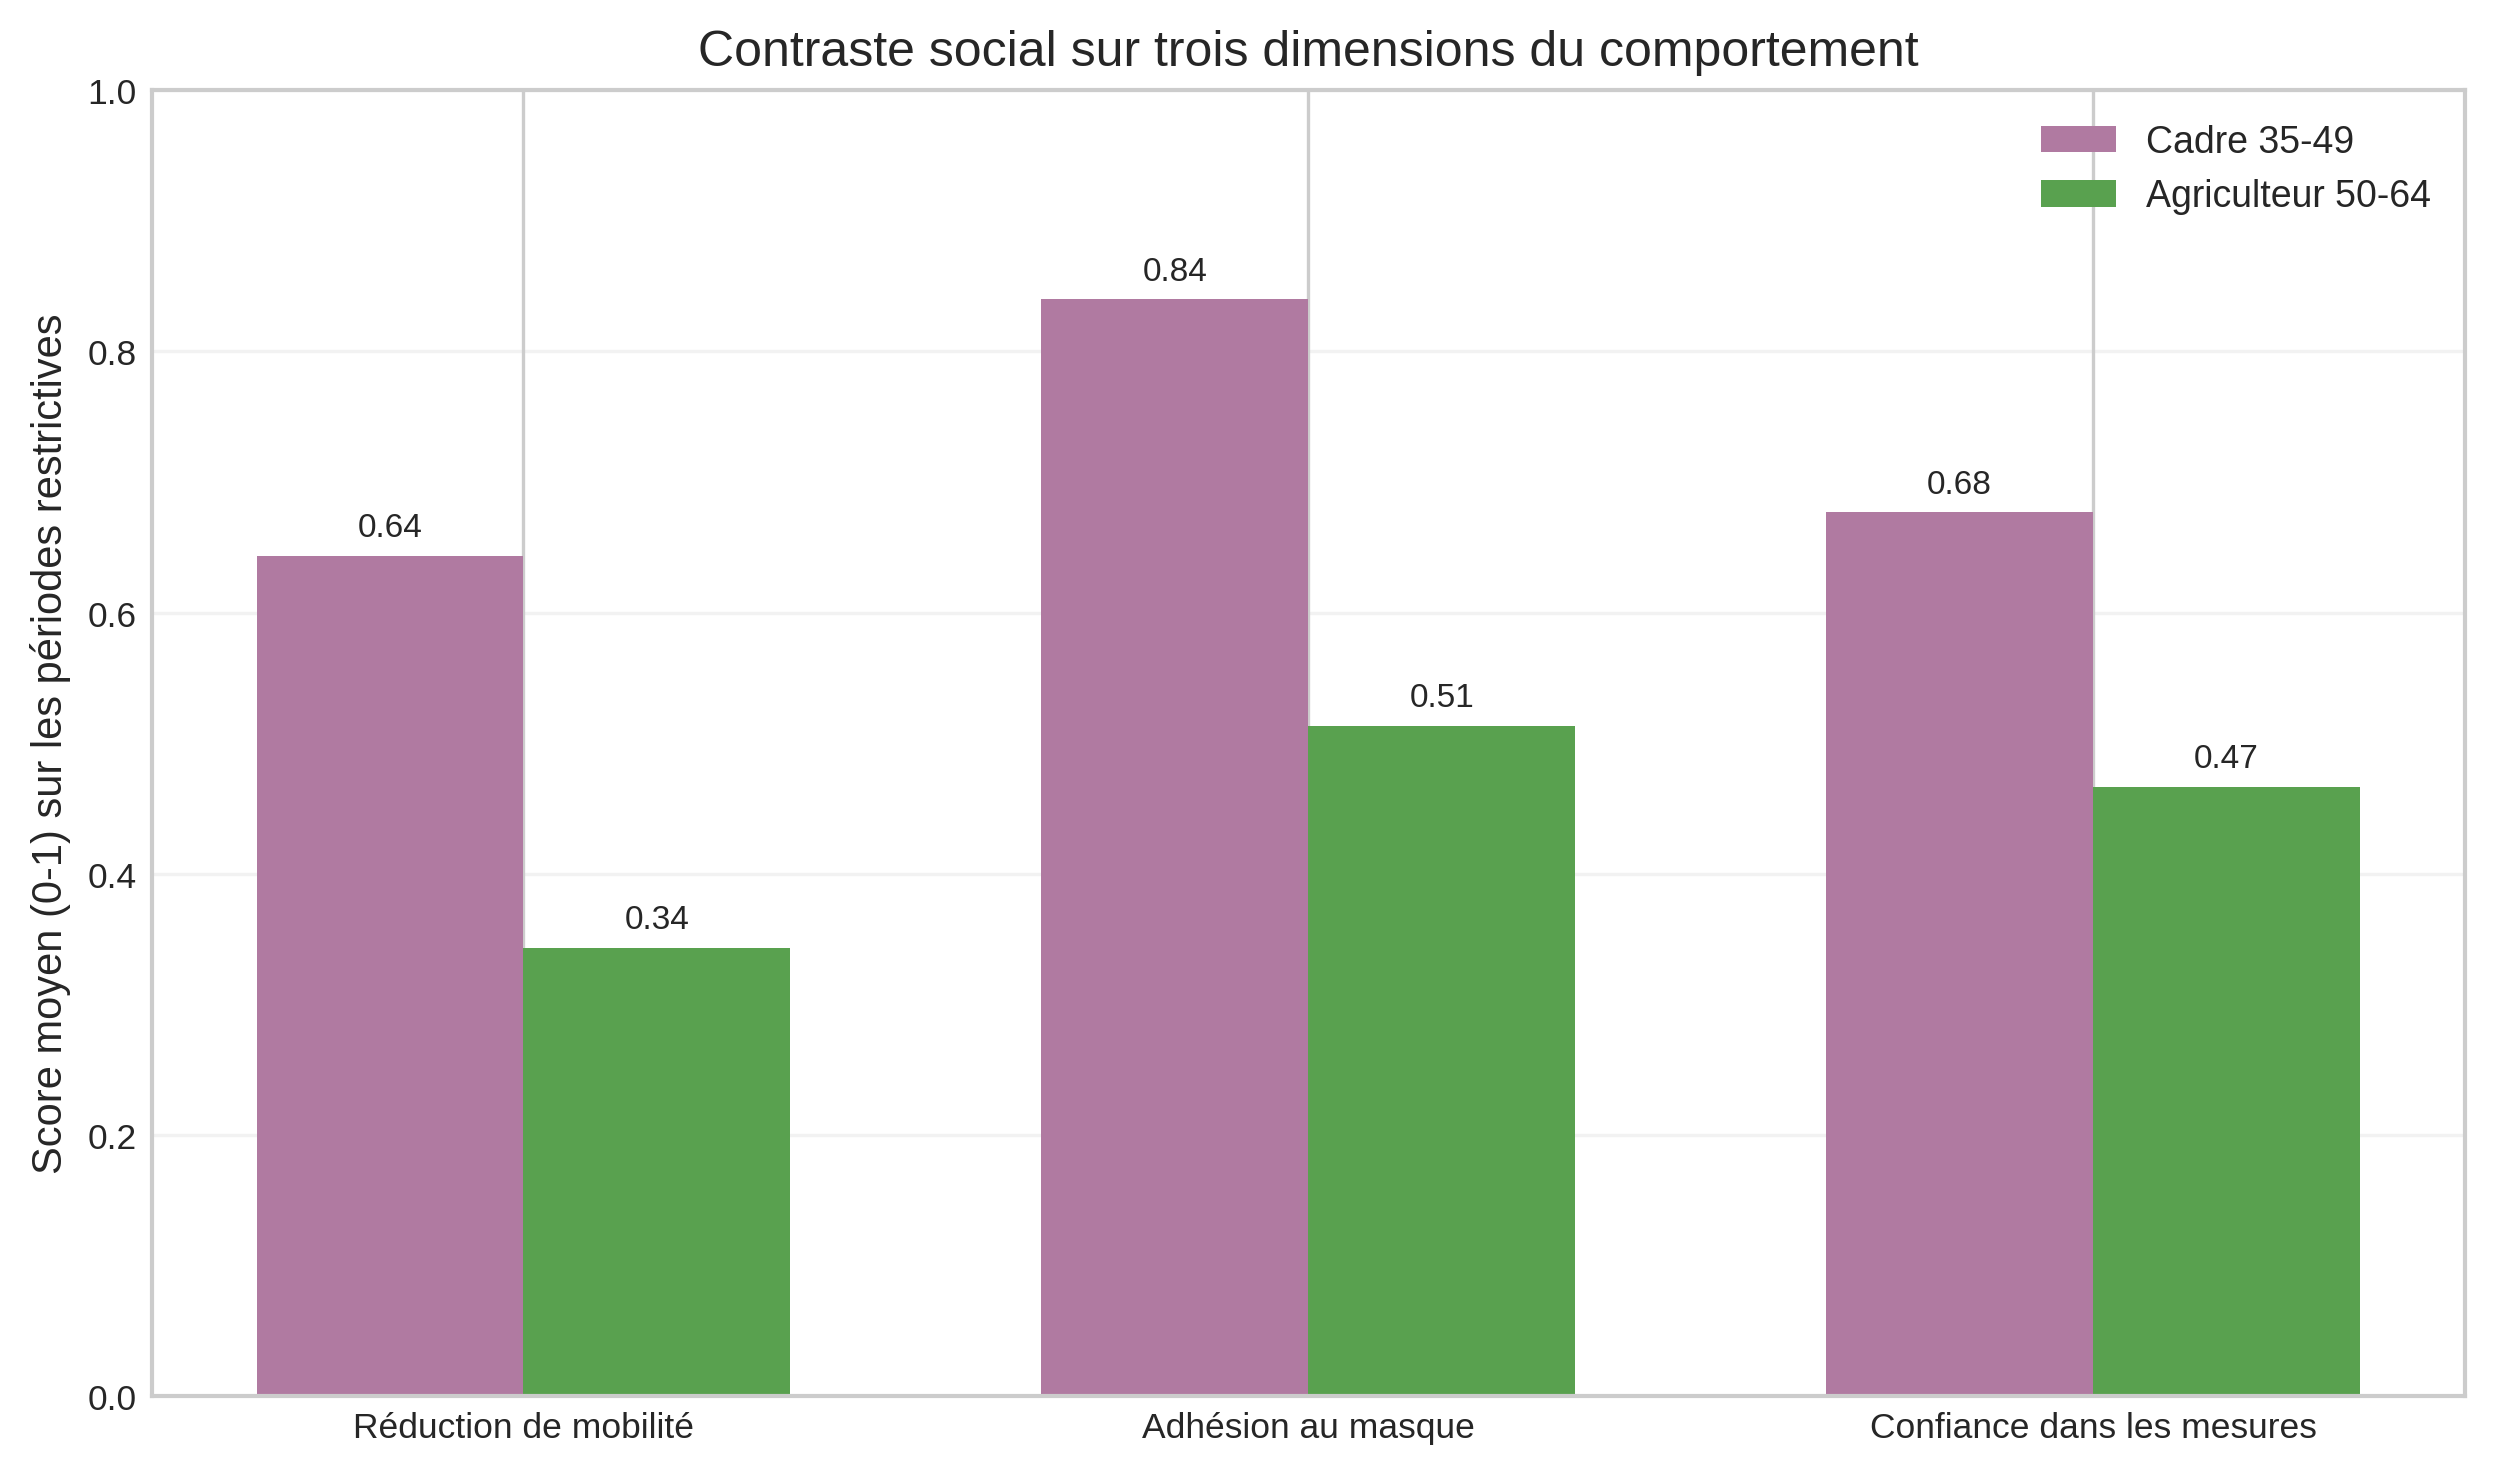
\includegraphics[width=0.78\textwidth]{figures/exp006_social_bias_analysis.png}
    \caption{Contraste de comportement entre un profil cadre et un profil agricole sur les périodes les plus restrictives.}
    \label{fig:exp006-bias}
\end{figure}

\subsection{Résultat principal : exp007 à exp009 transforment le bloc LLM en médiateur SHS défendable}
La séquence \texttt{exp007}, \texttt{exp008} et \texttt{exp009} constitue le résultat principal de cette version du papier. Elle ne doit pas être lue comme un détail d'implémentation, mais comme une expérience méthodologique sur la manière d'intégrer un LLM dans la chaîne de modélisation. Dans \texttt{exp007}, le médiateur SHS produit déjà un meilleur signal de prévention que l'heuristique, avec une MAE de 0,072 contre 0,141. En revanche, la mobilité échoue encore nettement, avec une MAE de 0,232 et une corrélation de 0,851, contre 0,094 et 0,863 pour la baseline heuristique. Le constat important est donc asymétrique : l'idée de médiation fonctionne partiellement, mais la variable latente de mobilité reste mal cadrée.

\texttt{Exp008} joue alors le rôle d'expérience de diagnostic. En ancrant explicitement la composante mobilité, on obtient une MAE de 0,002 et une corrélation quasi parfaite à 0,999. Cette expérience n'est pas présentée comme un modèle rival, mais comme une borne analytique montrant que l'échec de \texttt{exp007} vient bien de la spécification de \emph{mobility\_reduction} et non d'une impossibilité structurelle de la couche SHS/LLM à mieux faire que l'heuristique.

La campagne finale \texttt{exp009} corrige précisément ce point. Elle conserve la logique de médiation SHS, mais remplace le protocole initial par un prompt révisé centré sur la mobilité et exécute la campagne finale sur Claude Haiku 4.5. Le résultat est nettement plus fort : la MAE mobilité descend à 0,0219, contre 0,0935 pour l'heuristique, et la corrélation mobilité monte à 0,989, contre 0,863 pour la baseline. Le gain sur la prévention est conservé, avec une MAE de 0,0685 contre 0,1409. Le bloc LLM ne se contente donc plus de produire des profils socialement plausibles. Il devient capable, dans sa configuration finale, de surpasser la référence heuristique sur deux dimensions agrégées importantes.

\begin{table}[ht]
    \centering
    \footnotesize
    \caption{Progression du bloc SHS/LLM entre les campagnes récentes. L'expérience exp008 sert surtout de diagnostic sur l'ancrage mobilité et n'est donc pas directement comparable sur la prévention.}
    \resizebox{\linewidth}{!}{%
    \begin{tabular}{llrrr}
        \toprule
        Campagne & Modèle & MAE mobilité & Corrélation mobilité & MAE prévention \\
        \midrule
        Référence heuristique & Heuristique & 0{,}0935 & 0{,}863 & 0{,}1409 \\
        Exp007 initiale & Sonnet 4.6 & 0{,}2320 & 0{,}851 & 0{,}0724 \\
        Exp008 diagnostic & Ancrage & 0{,}0022 & 0{,}9998 & --- \\
        Exp009 finale & Haiku 4.5 & 0{,}0219 & 0{,}989 & 0{,}0685 \\
        \bottomrule
    \end{tabular}}
    \label{tab:llm-progression}
\end{table}

Le sens de cette progression dépasse le simple gain numérique. Elle montre que l'intégration des LLM dans l'étude n'est pas un ajout cosmétique. Le papier documente un passage méthodique entre une première campagne de profils plausibles, une reformulation médiatrice plus ambitieuse, un échec partiel localisé, puis une correction substantielle qui rend le bloc central scientifiquement défendable. C'est cette chaîne d'argumentation, davantage qu'un score isolé, qui lui donne sa cohérence.

\section{Discussion}
Le principal changement conceptuel est le suivant : le centre du papier n'est plus le seul socle statique, mais la manière dont une couche SHS/LLM peut venir s'y brancher sans perdre en lisibilité. Le socle statique demeure important, car il fournit un point d'ancrage transparent et robuste. La couche temporelle garde une utilité descriptive. Mais le résultat le plus intéressant, pour l'interface entre IA, SHS et épidémiologie, est la possibilité de faire jouer au LLM un rôle de médiateur socio-comportemental explicite plutôt que de simple générateur de texte ou de scores bruts.

Cette manière de cadrer le résultat rapproche davantage le papier des usages les plus prudents aujourd'hui discutés en sciences sociales computationnelles. Des travaux récents montrent que les LLM peuvent devenir utiles comme instruments d'annotation, de simulation contrainte ou de génération d'hypothèses, mais à condition de rester enchâssés dans des protocoles d'évaluation explicites et dans des tâches bien bornées \citep{argyle2023out,park2023generative,horton2023homo,ziems2024css}. Notre contribution s'inscrit plus clairement dans cette ligne : le modèle n'est ni traité comme oracle social, ni laissé libre de produire seul la structure du phénomène étudié. Il est mobilisé comme une couche médiatrice supplémentaire, adossée à des profils nommés, à des régimes historiques documentés et à des contrôles non LLM.

La séquence exp006 à exp009 clarifie aussi un point méthodologique plus général. Un bloc LLM ne doit pas être évalué comme s'il s'agissait d'un module monolithique. Les résultats dépendent fortement du niveau d'abstraction des profils, de la variable de sortie choisie, du prompt, de la manière dont cette sortie est réinjectée dans le pipeline, et du modèle mobilisé. Sous cet angle, l'échec partiel d'\texttt{exp007} est aussi instructif que le succès d'\texttt{exp009}. Il montre que le mauvais cadrage d'une variable latente peut annuler une partie du signal utile, alors même que la structure SHS générale est pertinente. Inversement, la forte amélioration d'\texttt{exp009} indique qu'une bonne partie du gain provient de l'articulation entre modèle, prompt et couche de projection, pas d'un simple effet de marque ou de taille du LLM.

Le fait d'avoir obtenu la campagne finale sur Claude Haiku 4.5 est ici intéressant en soi. Il suggère qu'un modèle plus léger peut rester scientifiquement utile lorsqu'il est inséré dans un protocole bien contraint, avec sorties structurées, profils explicites et comparaison à des baselines non LLM. Ce point rejoint un constat plus large de la littérature récente : la valeur scientifique de ces modèles est souvent très dépendante de la tâche, du protocole d'élicitation et du cadre de validation, bien plus que d'une hiérarchie abstraite entre modèles \citep{ziems2024css}. Cela ouvre une perspective naturelle pour la suite du travail : tester d'autres familles de LLM, comparer plus systématiquement des modèles généralistes et des modèles plus compacts, puis explorer des variantes fine-tunées ou instruction-tunées sur des sorties socio-comportementales structurées. Dans un tel programme, l'enjeu n'est pas seulement la performance brute. Il est aussi de mieux séparer l'effet du modèle, l'effet du prompt et l'effet de la couche de médiation elle-même.

Cette ouverture doit néanmoins rester prudente. Le simulateur ne découvre pas des essences sociales. Il réarticule des hypothèses de classe, de travail, de logement, de confiance et de contrainte de mobilité que nous avons explicitement encodées, puis que le modèle de langage réordonne. Le contraste cadres-agriculteurs, très visible dans les sorties, est donc intéressant parce qu'il rend les hypothèses distributives du pipeline audibles et discutables. Il ne doit pas être naturalisé comme une mesure définitive des groupes sociaux français. Cette prudence rejoint les mises en garde de la littérature sur les risques de stéréotypisation et de sur-interprétation des grands modèles de langage \citep{weidinger2022taxonomy,bender2021stochastic}.

Au total, la contribution du papier peut maintenant être formulée plus nettement. Nous ne proposons ni un substitut aux enquêtes françaises, ni une simulation sociale complète. Nous montrons qu'il est possible d'insérer, dans un pipeline français de matrices de contact, une couche SHS/LLM auditée, comparée à des contrôles explicites, et suffisamment performante dans sa version finale pour battre une heuristique sur la mobilité et la prévention agrégées. Le résultat reste borné, mais il devient plus intéressant : ce n'est plus seulement un article sur un bon baseline, c'est un article sur les conditions sous lesquelles l'intégration de LLM dans une étude épidémiologique peut devenir méthodologiquement crédible.

\section{Limites}
La première limite est la plus évidente : le socle statique reste agrégé à 17 classes d'âge et à une seule matrice nationale. Cette représentation efface des hétérogénéités importantes, qu'elles soient territoriales, intra-ménage, calendaires ou professionnelles. Elle reste adaptée à un protocole de contrôle, mais elle deviendrait insuffisante pour traiter des politiques localisées ou des scénarios fins.

Une deuxième limite concerne la couche temporelle. Malgré des gains réels sur l'indice de prévention, les résultats hors échantillon restent fragiles sur SocialCov, et certaines ablations simples améliorent encore la MAE de test. La partie dynamique du pipeline reste donc plus démonstrative qu'aboutie.

Une troisième limite tient au statut des profils SHS. Les 18 profils-situations sont des objets analytiques construits à partir de marges publiques, de sources INSEE, de proxys de télétravail et d'indices comportementaux raisonnés. Ils sont utiles pour rendre les hypothèses discutables, mais ils ne constituent pas des observations individuelles. Les écarts entre profils doivent être lus comme des scénarios structurés, non comme des estimations directes par catégorie socio-professionnelle.

Une quatrième limite concerne la validation externe du bloc LLM. Les cibles utilisées pour la prévention et pour l'alignement des profils restent partielles, car les données publiques disponibles ne fournissent pas une stratification complète et homogène par PCS sur l'ensemble des dimensions mobilisées. Le papier montre donc surtout une cohérence agrégée et une cohérence interne des sorties, plus qu'une validation forte sur comportements observés profil par profil.

Une cinquième limite est spécifique à la séquence exp007 à exp009. Le résultat final d'\texttt{exp009} est fort, mais il n'épuise pas la question du choix de modèle. Nous comparons ici peu de familles de LLM, et l'amélioration observée combine à la fois un changement de protocole de prompt et un changement de modèle. Il serait donc prématuré de conclure qu'un modèle donné domine structurellement un autre. La prochaine étape raisonnable consiste précisément à factoriser ce plan d'expériences en benchmark multi-modèles et en ablations de prompts, puis, si cela se confirme, en variantes fine-tunées sur sorties socio-comportementales structurées. C'est aussi le sens des recommandations formulées dans la littérature récente en sciences sociales computationnelles, qui insiste sur l'évaluation comparative plutôt que sur les démonstrations ad hoc \citep{ziems2024css}.

Une sixième limite touche à la reproductibilité réseau du bloc LLM. Les sorties archivées permettent de reproduire exactement les tableaux et figures retenus, mais une régénération en ligne dépend d'un accès configuré et d'une génération non strictement semée côté fournisseur. La traçabilité des artefacts est bonne. La réplication de la génération brute reste plus faible que celle des blocs purement déterministes.

Enfin, l'évaluation globale mobilise encore un nombre limité de métriques. MAE, distance de Frobenius, corrélation, assortativité locale et accord directionnel donnent une lecture utile, mais partielle. D'autres critères seraient nécessaires pour soutenir des affirmations plus fortes, par exemple l'impact sur un modèle épidémique aval, la sensibilité à un autre binning d'âge, ou la robustesse à des perturbations systématiques des profils et des politiques publiques.

\section{Conclusion}
Le manuscrit conduit à une lecture plus nette du projet. Le socle statique optimisé sur COMES-F reste utile et scientifiquement solide. La couche temporelle apporte un éclairage intéressant sur certaines séries françaises, tout en restant fragile hors échantillon. Mais l'apport central du papier se situe dans l'intégration d'une couche SHS/LLM explicite, progressive et auditée au sein d'un pipeline français de matrices de contact.

Ce point est important parce qu'il ne repose pas sur un seul résultat spectaculaire isolé. Il repose sur une trajectoire expérimentale lisible. Une première campagne sur Claude Sonnet 4.6 montre qu'un LLM profilé peut déjà restituer un ordre plausible des régimes sanitaires et des écarts sociaux de réactivité. Une seconde séquence, exp007 à exp009, met en évidence le verrou principal, le corrige, puis aboutit à une configuration finale sur Claude Haiku 4.5 qui surpasse l'heuristique à la fois sur la mobilité agrégée et sur la prévention. Le résultat le plus utile n'est donc pas seulement une amélioration de score. C'est la démonstration qu'une couche LLM peut devenir méthodologiquement crédible si elle est bornée, comparée, diagnostiquée et réinjectée proprement dans un cadre de modélisation.

Dans cette perspective, le papier ne doit pas être lu comme une promesse de remplacement des enquêtes ni comme une preuve de validité comportementale forte. Il doit être lu comme une proposition de méthode : comment relier des profils sociaux nommés, des régimes de politique publique et des modificateurs de contact épidémiologiquement pertinents, tout en gardant chaque hypothèse visible. C'est cette transparence, plus encore que la performance brute, qui rend l'article utile aujourd'hui et qui ouvre la suite logique du projet vers des comparaisons multi-LLM, des protocoles plus systématiques et, éventuellement, des modèles fine-tunés sur sorties socio-comportementales structurées.

% Auto-generated from src/contact_matrix_fr/agent_profiles.py
{\tiny
\setlength{\LTleft}{0pt}
\setlength{\LTright}{0pt}
\renewcommand{\arraystretch}{1.03}
\begin{longtable}{@{}>{\raggedright\arraybackslash}p{0.17\linewidth}>{\raggedright\arraybackslash}p{0.43\linewidth}ccc@{}}
\caption{Profils socio-démographiques utilisés dans l'expérience Exp006. Les colonnes \texttt{trust\_proxy}, multiplicateur préventif et contrainte de mobilité sont des paramètres synthétiques bornés entre 0 et 1.}\label{tab:profiles}\\
\toprule
Clé & Description synthétique & Trust & Prévention & Mobilité \\
\midrule
\endfirsthead
\toprule
Clé & Description synthétique & Trust & Prévention & Mobilité \\
\midrule
\endhead
\midrule
\multicolumn{5}{r}{\emph{Suite page suivante}}\\
\endfoot
\bottomrule
\endlastfoot
\path{etudiant_18_24_parents} & Étudiant 18-24 vivant chez ses parents (etudiant, chez parents) & 0.50 & 0.97 & 0.46 \\
\path{etudiant_18_24_colocation} & Étudiant 18-24 en colocation ou studio (etudiant, colocation ou studio) & 0.47 & 0.95 & 0.50 \\
\path{employe_25_34_seul} & Employé 25-34 vivant seul (employe, seul) & 0.49 & 0.99 & 0.74 \\
\path{employe_35_49_monoparent} & Employé 35-49 en famille monoparentale (employe, famille monoparentale) & 0.46 & 0.98 & 0.78 \\
\path{ouvrier_25_34_couple_enfants} & Ouvrier 25-34 en couple avec enfants (ouvrier, couple avec enfants) & 0.43 & 0.96 & 0.84 \\
\path{ouvrier_35_49_couple_enfants} & Ouvrier 35-49 en couple avec enfants (ouvrier, couple avec enfants) & 0.41 & 0.96 & 0.85 \\
\path{employe_35_49_couple_enfants} & Employé 35-49 en couple avec enfants (employe, couple avec enfants) & 0.50 & 1.00 & 0.72 \\
\path{profession_intermediaire_35_49_couple_enfants} & Profession intermédiaire 35-49 en couple avec enfants (profession intermediaire, couple avec enfants) & 0.58 & 1.02 & 0.58 \\
\path{cadre_25_34_seul} & Cadre 25-34 vivant seul (cadre, seul) & 0.65 & 1.05 & 0.34 \\
\path{cadre_35_49_couple_enfants} & Cadre 35-49 en couple avec enfants (cadre, couple avec enfants) & 0.68 & 1.06 & 0.38 \\
\path{independant_35_49_couple_enfants} & Indépendant 35-49 en couple avec enfants (artisan commercant, couple avec enfants) & 0.42 & 0.95 & 0.70 \\
\path{agriculteur_50_64_couple} & Agriculteur 50-64 en couple (agriculteur, couple) & 0.48 & 0.98 & 0.72 \\
\path{inactif_50_64_seul} & Inactif 50-64 vivant seul (inactive au foyer, seul) & 0.51 & 1.01 & 0.44 \\
\path{chomeur_25_49_seul} & Chômeur 25-49 vivant seul ou chez un proche (chomeur, seul ou heberge) & 0.39 & 0.94 & 0.40 \\
\path{retraite_65_74_couple} & Retraité 65-74 en couple (retraite, couple) & 0.64 & 1.08 & 0.42 \\
\path{retraite_75_plus_seul} & Retraité 75+ vivant seul (retraite, seul) & 0.66 & 1.10 & 0.34 \\
\path{employe_50_64_couple} & Employé 50-64 en couple (employe, couple) & 0.54 & 1.03 & 0.66 \\
\path{ouvrier_50_64_couple} & Ouvrier 50-64 en couple (ouvrier, couple) & 0.44 & 0.99 & 0.80 \\
\end{longtable}
}


\section*{Disponibilité des données et du code}
L'ensemble du code, des configurations d'expériences, des artefacts JSON et des scripts de génération de figures est distribué publiquement sous licence MIT. Les données empiriques externes, notamment COMES-F, CoviPrev, SocialCov et Google Community Mobility Reports, restent accessibles via leurs dépôts d'origine et conservent leur licence respective. Les campagnes LLM retenues dans le manuscrit sont archivées sous forme de sorties JSON structurées, avec les agrégations et métadonnées nécessaires à la reproduction exacte des tableaux et figures. Une régénération en ligne du bloc LLM nécessite toutefois un environnement configuré et ne doit pas être confondue avec la reproduction exacte à partir des artefacts archivés.

\section*{Déclaration de conflit d'intérêts}
L'auteur déclare n'avoir aucun conflit d'intérêts en lien avec ce travail. Aucune rémunération n'a été perçue d'une organisation susceptible d'influencer la conduite de la recherche ou la rédaction du manuscrit.

\section*{Remerciements}
L'auteur remercie chaleureusement l'équipe pédagogique du Diplôme d'Université d'analyse des données de l'Université Paris 1 Panthéon-Sorbonne, qui, malgré les réorganisations et changements de direction survenus durant la formation, a su assurer un encadrement attentif et continu à l'ensemble de la promotion. L'auteur remercie également ses camarades de groupe, dont les discussions informelles ont nourri plusieurs pistes méthodologiques du projet.

\bibliography{roia_manuscript}

\end{document}
